\documentclass[
  shownotes,
  xcolor={svgnames},
  hyperref={colorlinks,citecolor=DarkBlue,linkcolor=andesred,urlcolor=DarkBlue}
  , aspectratio=169]{beamer}
\usepackage{animate}
\usepackage{amsmath}
\usepackage{amsfonts}
\usepackage{amssymb}
\usepackage{pifont}
\usepackage{mathpazo}
%\usepackage{xcolor}
\usepackage{multimedia}
\usepackage{fancybox}
\usepackage[para]{threeparttable}
\usepackage{multirow}
\setcounter{MaxMatrixCols}{30}
\usepackage{subcaption}
\usepackage{graphicx}
\usepackage{lscape}
\usepackage[compatibility=false,font=small]{caption}
\usepackage{booktabs}
\usepackage{ragged2e}
\usepackage{chronosys}
\usepackage{appendixnumberbeamer}
\usepackage{animate}
\setbeamertemplate{caption}[numbered]
\usepackage{color}
%\usepackage{times}
\usepackage{tikz}
\usetikzlibrary{arrows}
\usepackage{comment} %to comment
%% BibTeX settings
\usepackage{natbib}
\bibliographystyle{apalike}
\bibpunct{(}{)}{,}{a}{,}{,}
\setbeamertemplate{bibliography item}{[\theenumiv]}

% Defines columns for bespoke tables
\usepackage{array}
\newcolumntype{L}[1]{>{\raggedright\let\newline\\\arraybackslash\hspace{0pt}}m{#1}}
\newcolumntype{C}[1]{>{\centering\let\newline\\\arraybackslash\hspace{0pt}}m{#1}}
\newcolumntype{R}[1]{>{\raggedleft\let\newline\\\arraybackslash\hspace{0pt}}m{#1}}


\usepackage{xfrac}


\usepackage{multicol}
\setlength{\columnsep}{0.5cm}

% Theme and colors
\usetheme{Boadilla}

% I define a custom pallete
\definecolor{andesred}{HTML}{1B175E}
\definecolor{andesyellow}{HTML}{ffff00}

% Other options
\providecommand{\U}[1]{\protect\rule{.1in}{.1in}}
\usefonttheme{serif}
\setbeamertemplate{itemize items}[default]
\setbeamertemplate{enumerate items}[square]
\setbeamertemplate{section in toc}[circle]


\definecolor{mybackground}{HTML}{1B175E}
\definecolor{myforeground}{HTML}{0000A0}

\setbeamercolor{normal text}{fg=black,bg=white}
\setbeamercolor{alerted text}{fg=andesred}
\setbeamercolor{example text}{fg=black}

\setbeamercolor{background canvas}{fg=myforeground, bg=white}
\setbeamercolor{background}{fg=myforeground, bg=mybackground}
\setbeamercolor{palette tertiary}{fg=myforeground,bg=mybackground}

\setbeamercolor{palette primary}{fg=black, bg=white}
\setbeamercolor{palette secondary}{fg=black, bg=white!10!andesyellow}
\setbeamercolor{palette tertiary}{fg=black, bg=white}


\setbeamercolor{frametitle}{fg=black}
\setbeamercolor{title}{fg=black}
\setbeamercolor{block title}{fg=andesred}
\setbeamercolor{itemize item}{fg=andesred}
\setbeamercolor{itemize subitem}{fg=andesred}
\setbeamercolor{itemize subsubitem}{fg=andesred}
\setbeamercolor{enumerate item}{fg=andesred}
\setbeamercolor{item projected}{bg=gray!30!white,fg=andesred}
\setbeamercolor{enumerate subitem}{fg=andesred}
\setbeamercolor{section number projected}{bg=gray!30!white,fg=andesred}
\setbeamercolor{section in toc}{fg=andesred}
\setbeamercolor{caption name}{fg=andesred}
\setbeamercolor{button}{bg=gray!30!white,fg=andesred}
\setbeamercolor{title in head/foot}{fg=andesred}



\usepackage{fancyvrb}
\newcommand{\VerbBar}{|}
\newcommand{\VERB}{\Verb[commandchars=\\\{\}]}
\DefineVerbatimEnvironment{Highlighting}{Verbatim}{commandchars=\\\{\}}
% Add ',fontsize=\small' for more characters per line
\usepackage{framed}
\definecolor{shadecolor}{RGB}{248,248,248}
\newenvironment{Shaded}{\begin{snugshade}}{\end{snugshade}}
\newcommand{\AlertTok}[1]{\textcolor[rgb]{0.94,0.16,0.16}{#1}}
\newcommand{\AnnotationTok}[1]{\textcolor[rgb]{0.56,0.35,0.01}{\textbf{\textit{#1}}}}
\newcommand{\AttributeTok}[1]{\textcolor[rgb]{0.77,0.63,0.00}{#1}}
\newcommand{\BaseNTok}[1]{\textcolor[rgb]{0.00,0.00,0.81}{#1}}
\newcommand{\BuiltInTok}[1]{#1}
\newcommand{\CharTok}[1]{\textcolor[rgb]{0.31,0.60,0.02}{#1}}
\newcommand{\CommentTok}[1]{\textcolor[rgb]{0.56,0.35,0.01}{\textit{#1}}}
\newcommand{\CommentVarTok}[1]{\textcolor[rgb]{0.56,0.35,0.01}{\textbf{\textit{#1}}}}
\newcommand{\ConstantTok}[1]{\textcolor[rgb]{0.00,0.00,0.00}{#1}}
\newcommand{\ControlFlowTok}[1]{\textcolor[rgb]{0.13,0.29,0.53}{\textbf{#1}}}
\newcommand{\DataTypeTok}[1]{\textcolor[rgb]{0.13,0.29,0.53}{#1}}
\newcommand{\DecValTok}[1]{\textcolor[rgb]{0.00,0.00,0.81}{#1}}
\newcommand{\DocumentationTok}[1]{\textcolor[rgb]{0.56,0.35,0.01}{\textbf{\textit{#1}}}}
\newcommand{\ErrorTok}[1]{\textcolor[rgb]{0.64,0.00,0.00}{\textbf{#1}}}
\newcommand{\ExtensionTok}[1]{#1}
\newcommand{\FloatTok}[1]{\textcolor[rgb]{0.00,0.00,0.81}{#1}}
\newcommand{\FunctionTok}[1]{\textcolor[rgb]{0.00,0.00,0.00}{#1}}
\newcommand{\ImportTok}[1]{#1}
\newcommand{\InformationTok}[1]{\textcolor[rgb]{0.56,0.35,0.01}{\textbf{\textit{#1}}}}
\newcommand{\KeywordTok}[1]{\textcolor[rgb]{0.13,0.29,0.53}{\textbf{#1}}}
\newcommand{\NormalTok}[1]{#1}
\newcommand{\OperatorTok}[1]{\textcolor[rgb]{0.81,0.36,0.00}{\textbf{#1}}}
\newcommand{\OtherTok}[1]{\textcolor[rgb]{0.56,0.35,0.01}{#1}}
\newcommand{\PreprocessorTok}[1]{\textcolor[rgb]{0.56,0.35,0.01}{\textit{#1}}}
\newcommand{\RegionMarkerTok}[1]{#1}
\newcommand{\SpecialCharTok}[1]{\textcolor[rgb]{0.00,0.00,0.00}{#1}}
\newcommand{\SpecialStringTok}[1]{\textcolor[rgb]{0.31,0.60,0.02}{#1}}
\newcommand{\StringTok}[1]{\textcolor[rgb]{0.31,0.60,0.02}{#1}}
\newcommand{\VariableTok}[1]{\textcolor[rgb]{0.00,0.00,0.00}{#1}}
\newcommand{\VerbatimStringTok}[1]{\textcolor[rgb]{0.31,0.60,0.02}{#1}}
\newcommand{\WarningTok}[1]{\textcolor[rgb]{0.56,0.35,0.01}{\textbf{\textit{#1}}}}
\usepackage{graphicx}
\makeatletter

\makeatother





\AtBeginSection[]
{
    \begin{frame}
        \frametitle{Agenda}
        \tableofcontents[currentsection]
    \end{frame}
}



\AtBeginSubsection[]
{
    \begin{frame}
        \frametitle{Agenda}
        \tableofcontents[currentsubsection]
    \end{frame}
}


%%%%%%%%%%%%%%% BEGINS DOCUMENT %%%%%%%%%%%%%%%%%%


\begin{document}


\title{Spatial Data}
\subtitle{Big Data y Machine Learning para Economía Aplicada}
\date{}

\author[Sarmiento-Barbieri]{Ignacio Sarmiento-Barbieri}
\institute[Uniandes]{Universidad de los Andes}


\begin{frame}[noframenumbering]
\maketitle
\end{frame}





%----------------------------------------------------------------------% 

\begin{frame}
\frametitle{Agenda}

\tableofcontents

\end{frame}




%----------------------------------------------------------------------%
\section{Motivation }
%----------------------------------------------------------------------%


\begin{frame}[fragile]
\frametitle{Motivation}


\begin{itemize}
  \item In Big Data  volume was only a part of the story 
  \bigskip
  \item Big Data are data of high complexity: anarchic and spontaneous
  \bigskip
  \item They are the by product of an action: pay with credit card, tweet, move from point A to point B, buy a house, etc.
  \bigskip
  \item Now we are going to center on spatial data
\end{itemize}

\end{frame}


%----------------------------------------------------------------------%
\section{Types of Spatial Data}
%----------------------------------------------------------------------%
\begin{frame}[fragile]
\frametitle{Types of Spatial Data}
Spatial data comes in many ``shapes'' and ``sizes'', the most common types of spatial data are:
\medskip
\begin{itemize}
  \item Points are the most basic form of spatial data. Denotes a single point location, such as cities, a GPS reading or any other discrete object defined in space.
  \medskip
  \item Lines are a set of ordered points, connected by straight line segments
  \medskip
  \item Polygons denote an area, and can be thought as a sequence of connected points, where the first point is the same as the last
  \medskip
  \item Grid (Raster) are a collection of points or rectangular cells, organized in a regular lattice
\end{itemize}

\end{frame}
%----------------------------------------------------------------------%
\begin{frame}[fragile]
\frametitle{Types of Spatial Data: Points}

\begin{figure}[H] \centering
  
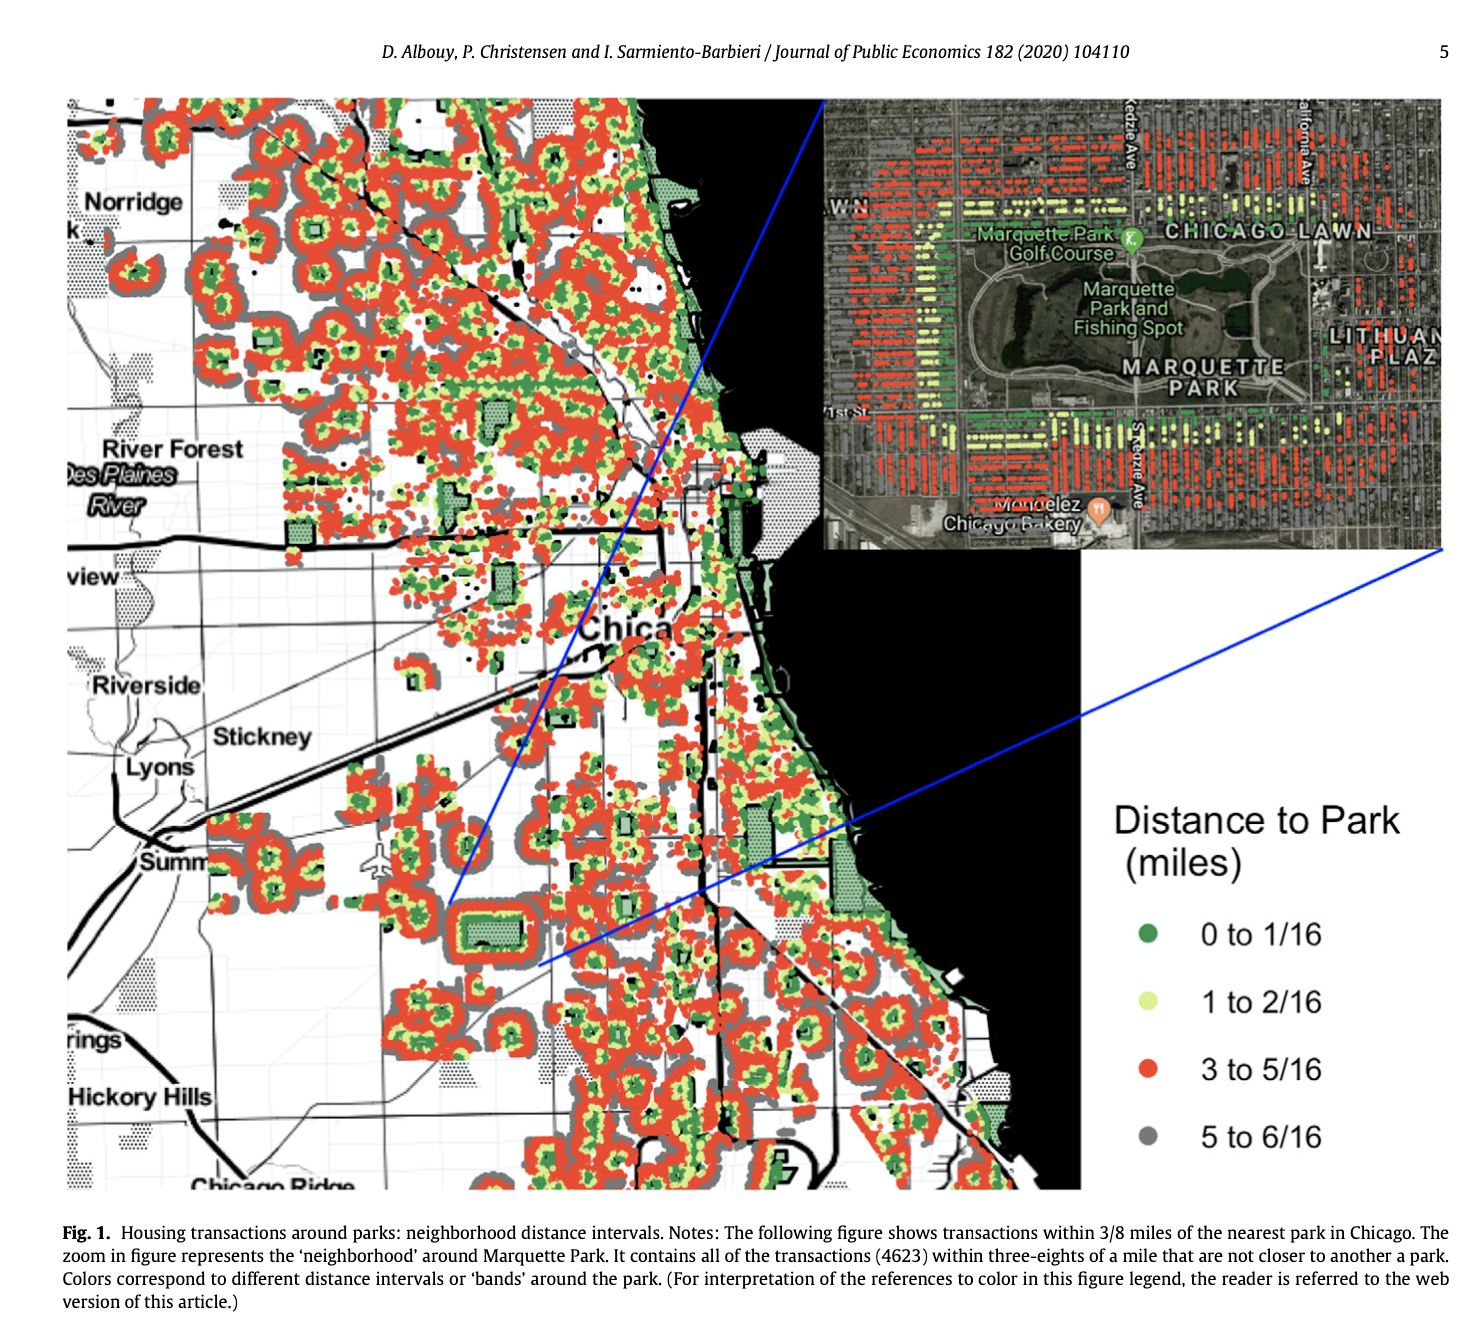
\includegraphics[scale=0.35]{figures/albouy_et_al_fig1.png}
  \\
  \tiny Albouy, Christensen \& Sarmiento-Barbieri (2020)
\end{figure}


\end{frame}

%----------------------------------------------------------------------%
\begin{frame}[fragile]
\frametitle{Types of Spatial Data: Lines}

\begin{figure}[H] 
  \centering
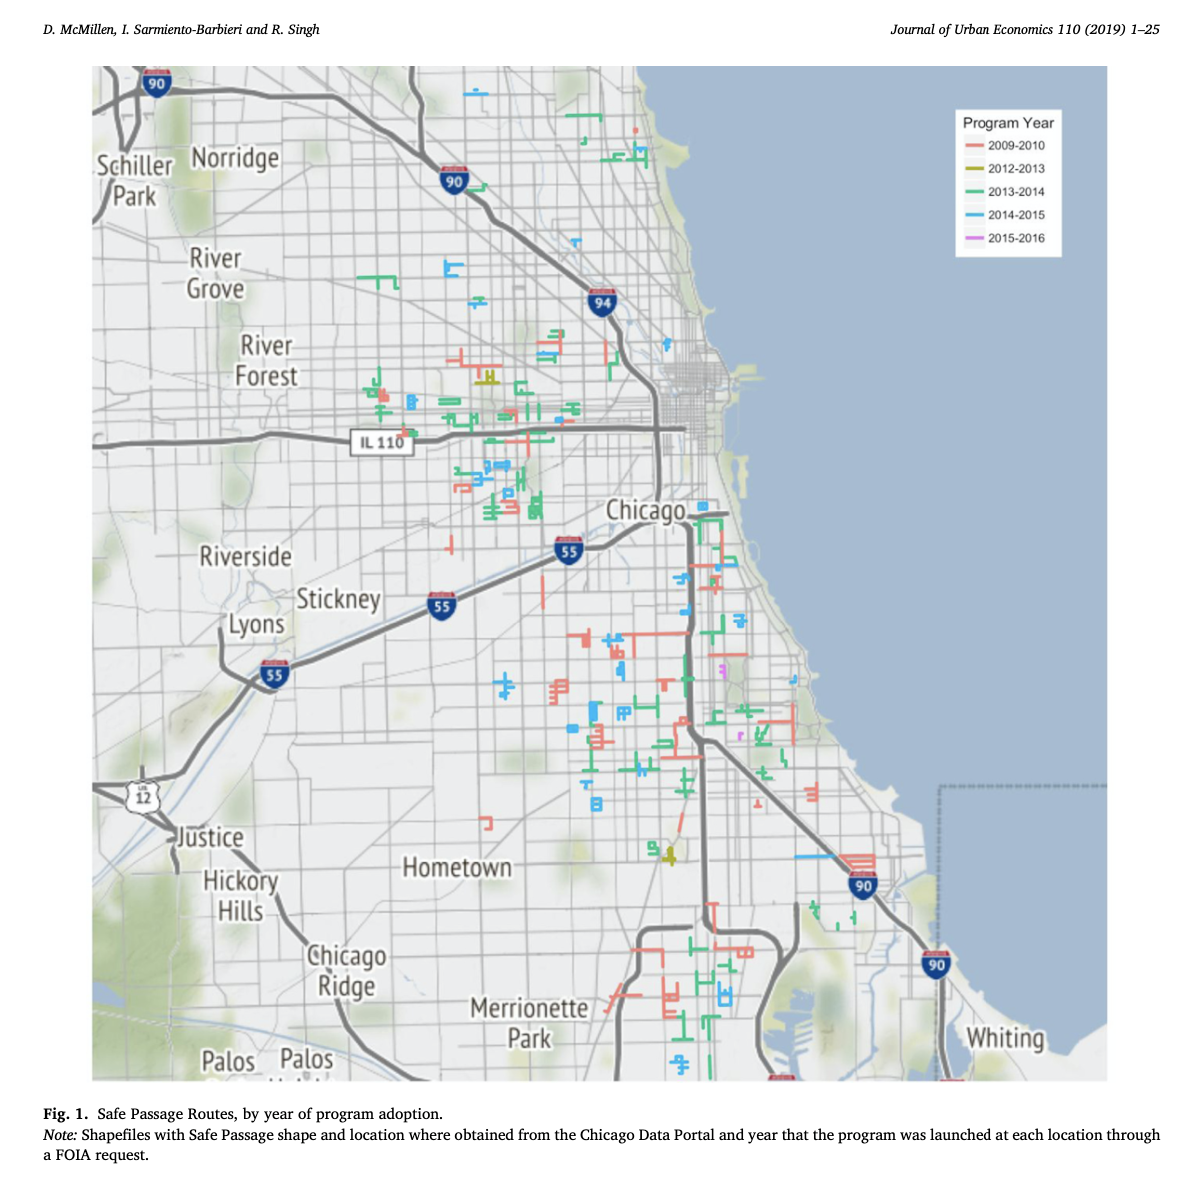
\includegraphics[scale=0.35]{figures/safe_passage.png}
  \\
\tiny McMillen, Sarmiento-Barbieri \& Singh, 2019

\end{figure}

\end{frame}

%----------------------------------------------------------------------%
\begin{frame}[fragile]
\frametitle{Types of Spatial Data: Polygons}

\begin{figure}[H] \centering
  \centering
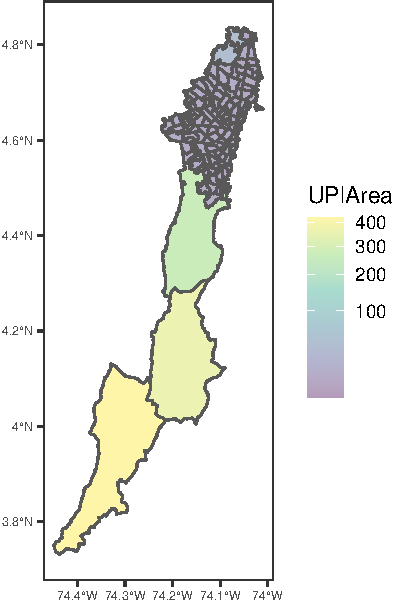
\includegraphics[scale=0.60]{figures/upz.pdf}
  \\
  \tiny Source:\url{https://datosabiertos.bogota.gov.co/dataset/unidad-de-planeamiento-bogota-d-c}
\end{figure}



\end{frame}

%----------------------------------------------------------------------%
\begin{frame}[fragile]
\frametitle{Types of Spatial Data: Rasters}

\begin{figure}[H] \centering
  \centering
  
\begin{subfigure}{0.45\linewidth}
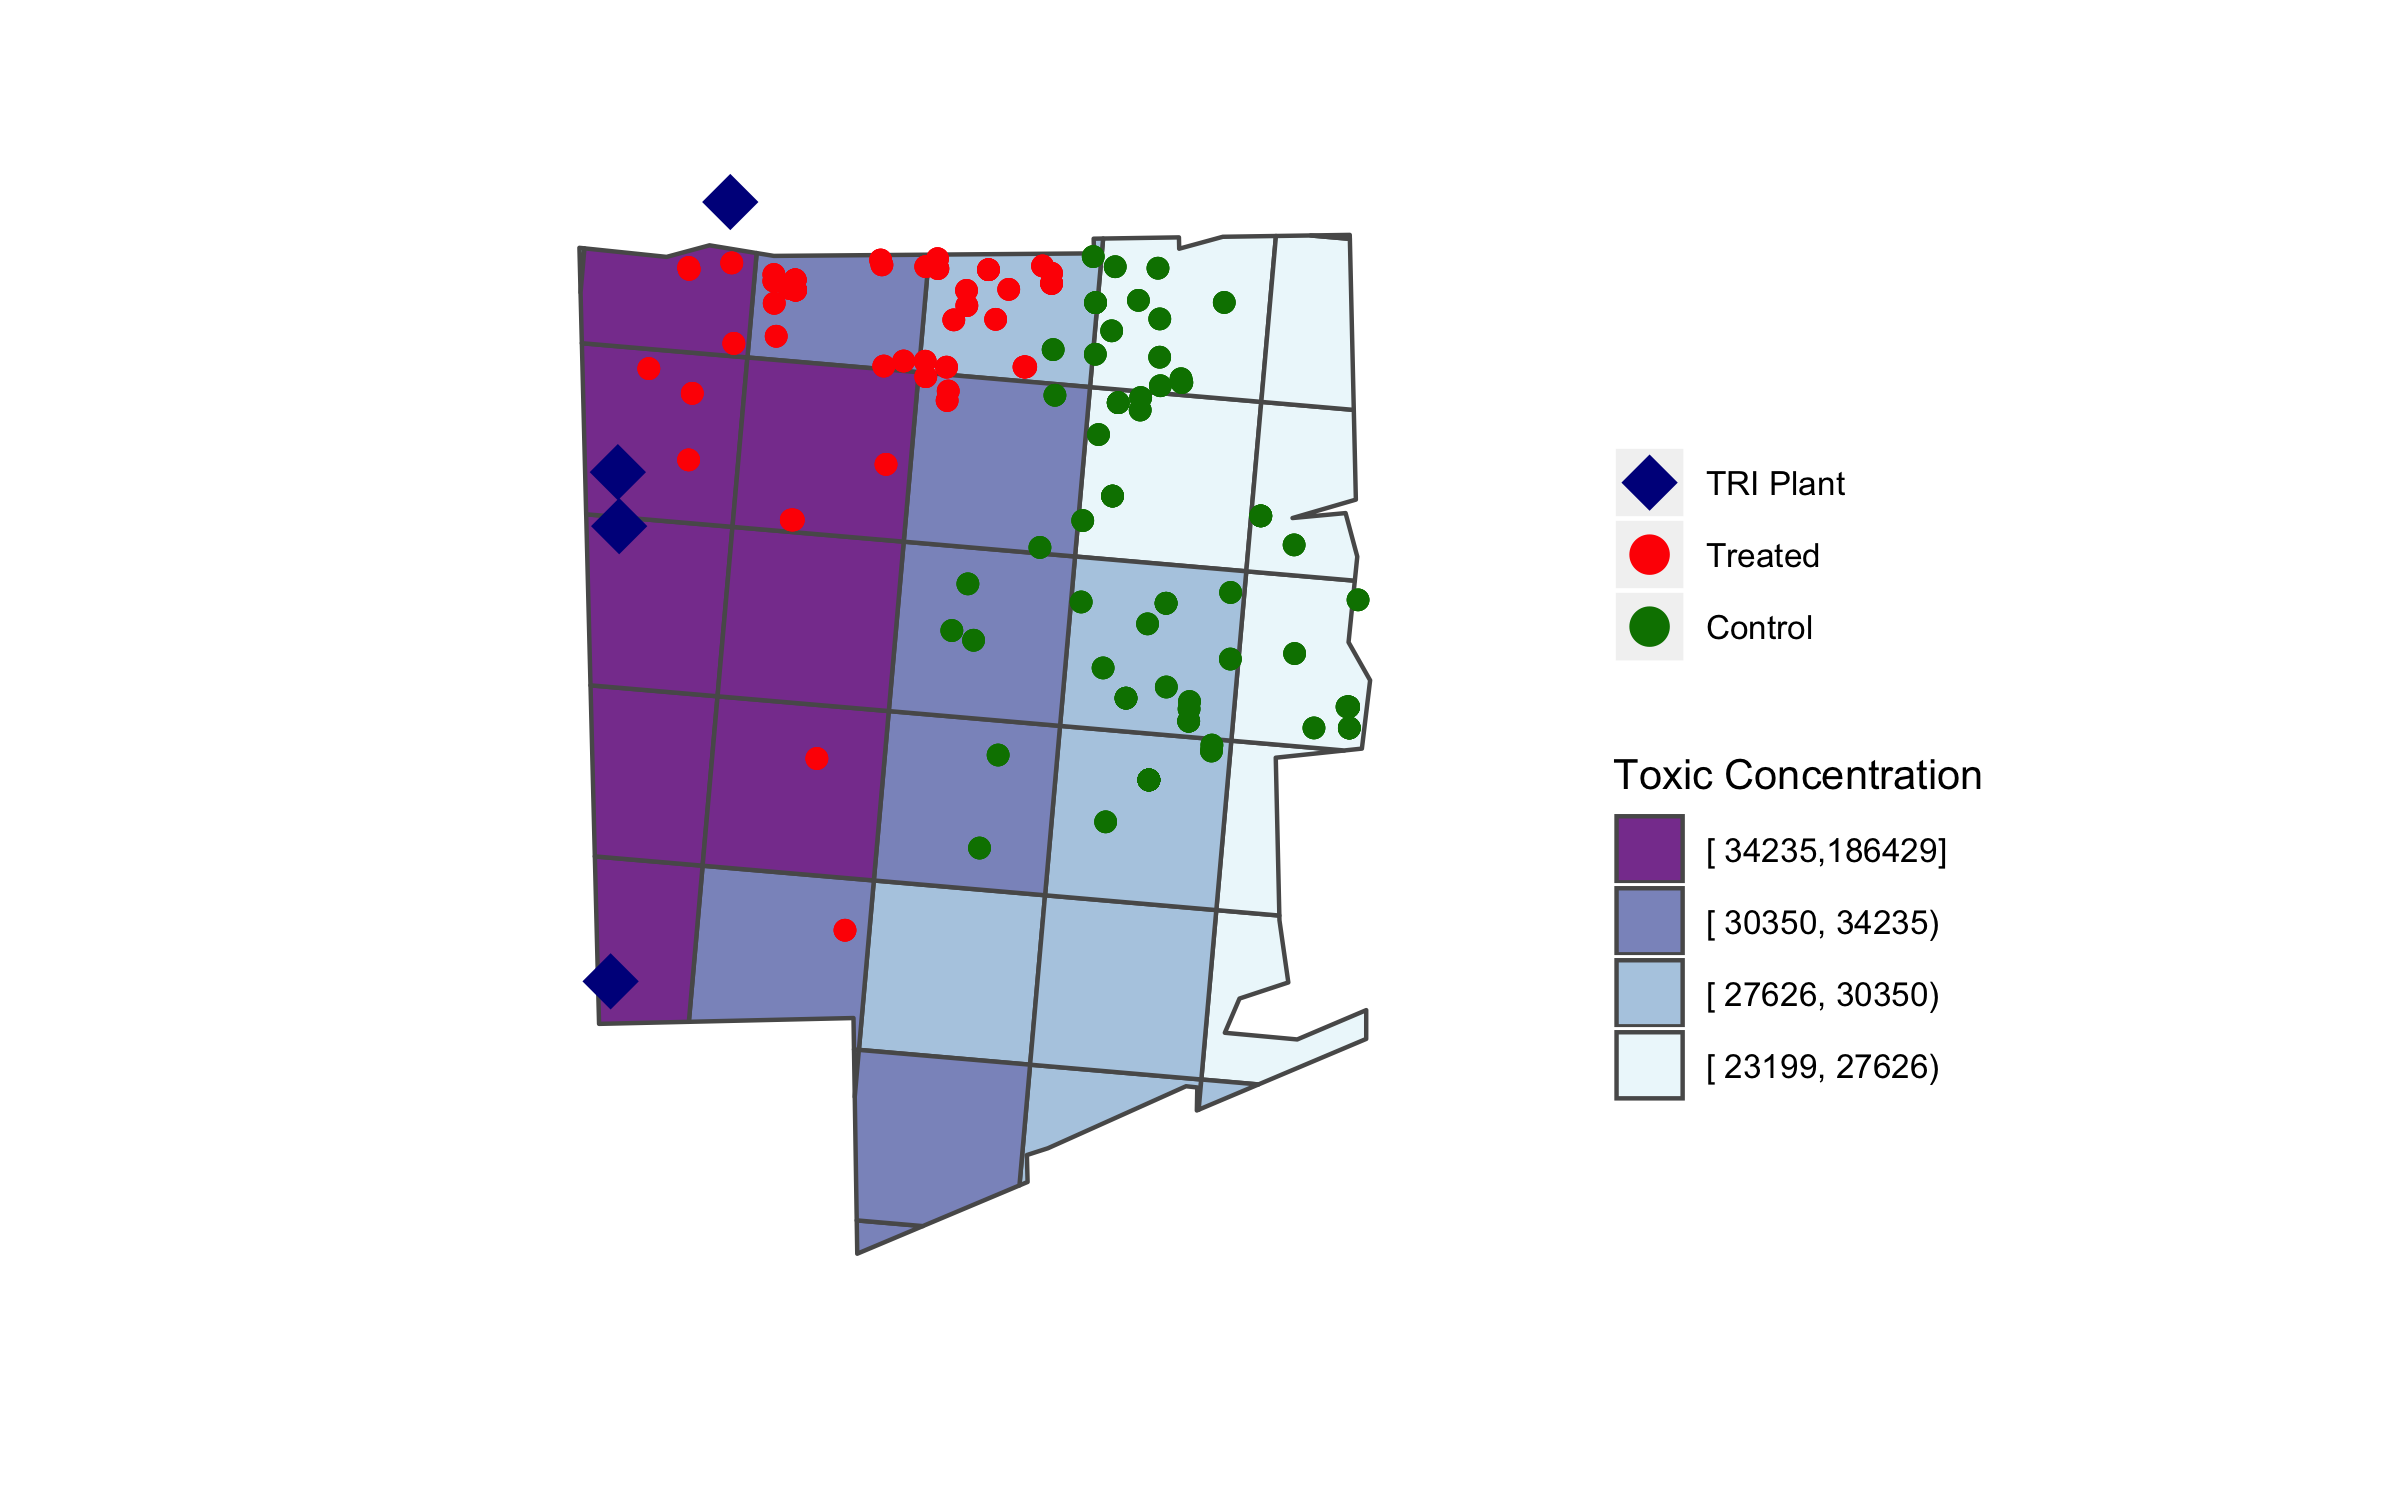
\includegraphics[scale=0.08]{figures/ZIP_A.png}
\end{subfigure}
\begin{subfigure}{0.45\linewidth}
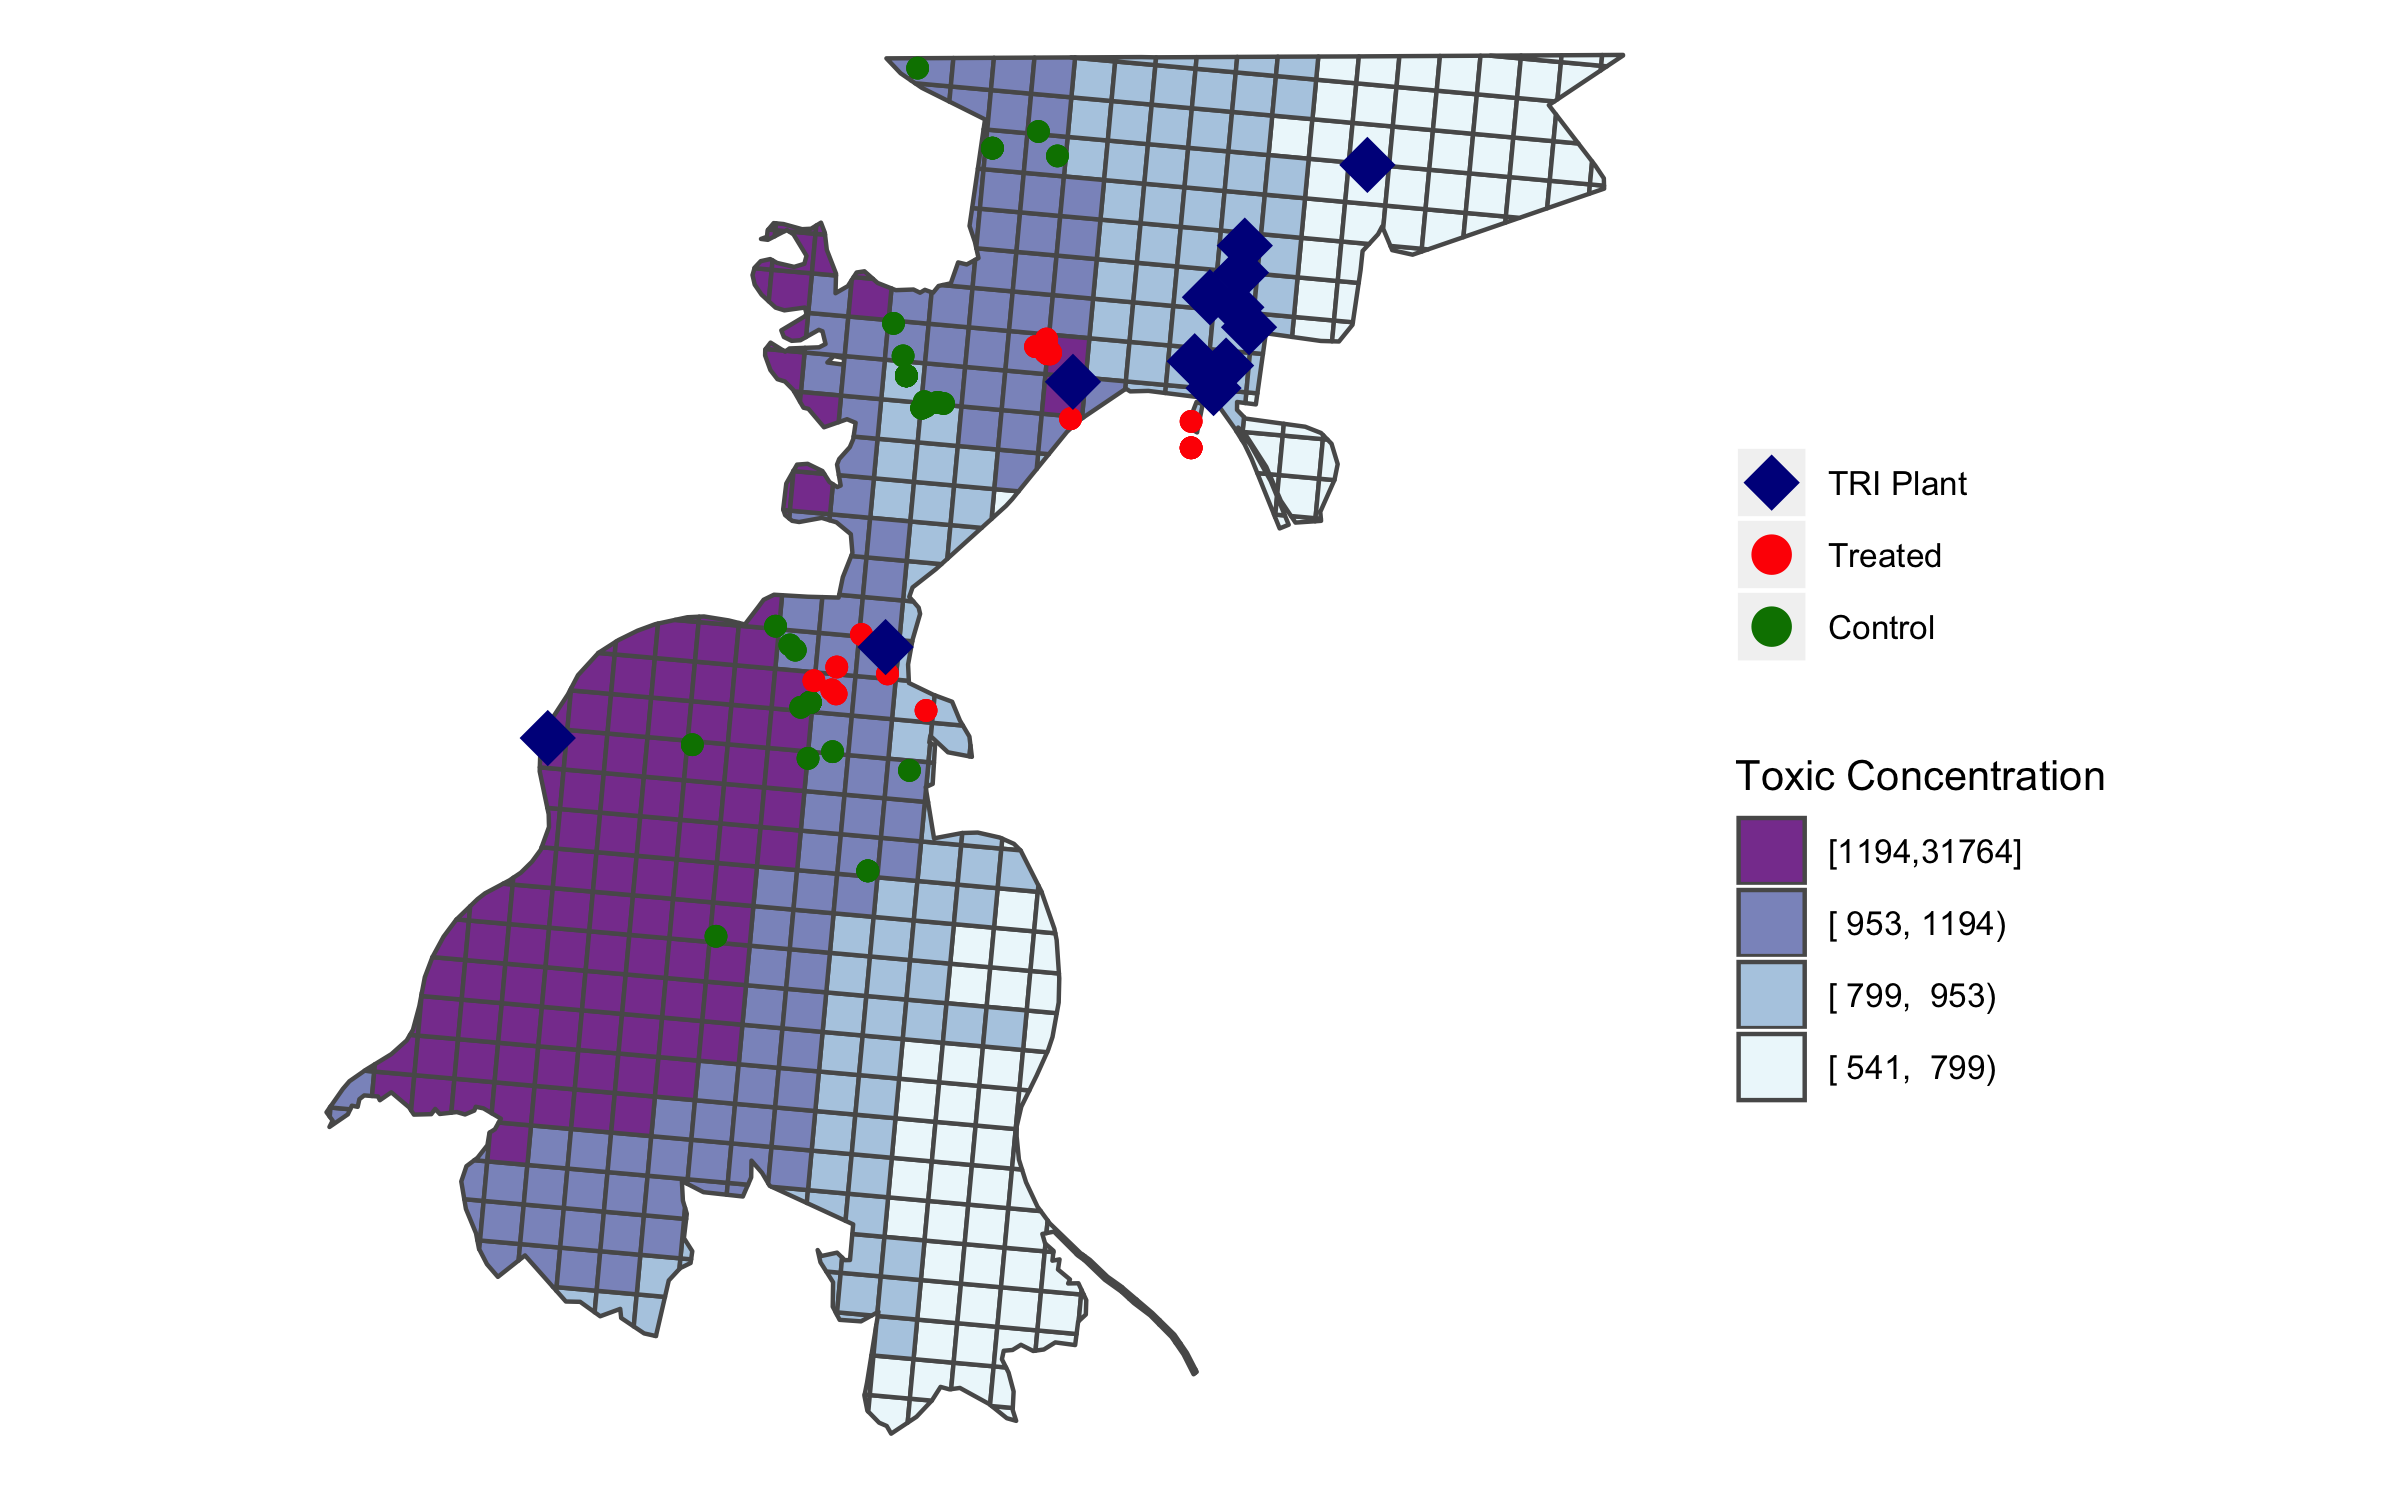
\includegraphics[scale=0.08]{figures/ZIP_B.png}

\end{subfigure}
  \\
  \tiny Christensen,Sarmiento-Barbieri  \& Timmins (2022)
\end{figure}


\end{frame}


%----------------------------------------------------------------------%
\section{Projections}
%----------------------------------------------------------------------%
\begin{frame}[fragile]
\frametitle{The earth ain't flat}
\begin{itemize}
  
  \item The world is an irregularly shaped ellipsoid, but plotting devices are flat
  \medskip
  \item But if you want to show it on a flat map you need a map projection, 
  \medskip
  \item This  will determine how to transform and distort latitudes and longitudes to preserve some of the map properties: area, shape, distance, direction or bearing
\end{itemize}

\end{frame}
%----------------------------------------------------------------------%
\begin{frame}[fragile]
\frametitle{The earth ain't flat}

\begin{itemize}
    \footnotesize
\item Map projections try to portray the surface of the earth or a portion of the earth on a flat piece of paper or computer screen. 
\medskip
\item A coordinate reference system (CRS) then defines, with the help of coordinates, how the two-dimensional, projected map in your GIS is related to real places on the earth. 
\end{itemize}

\begin{figure}[H] \centering
            \captionsetup{justification=centering}
                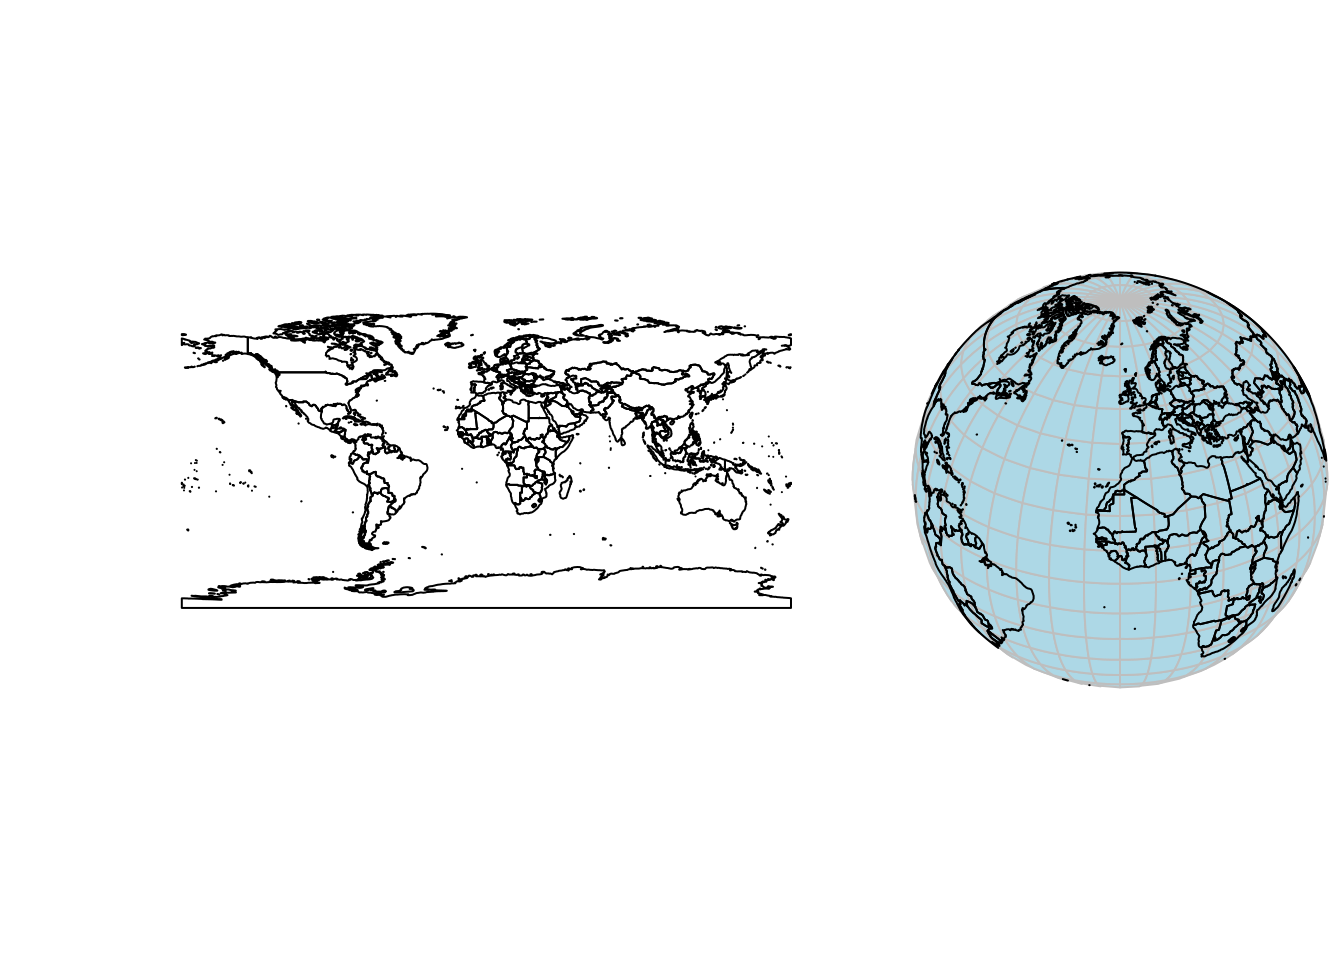
\includegraphics[scale=0.6]{figures/world-1.png}
 \end{figure}

\end{frame}
%----------------------------------------------------------------------%
\begin{frame}[fragile]
\frametitle{The earth ain't flat}
\begin{itemize}
  \footnotesize
  \item For example, sailors use Mercator projection where meridians and parallels cross each other always at the same 90 degrees angle.
  \medskip
  \item It allows to easy locate your self on the line showing direction in which you sail
  \medskip
  \item But the projection do not preserve  distances
\end{itemize}
 


\begin{figure}[H] \centering
            \captionsetup{justification=centering}
        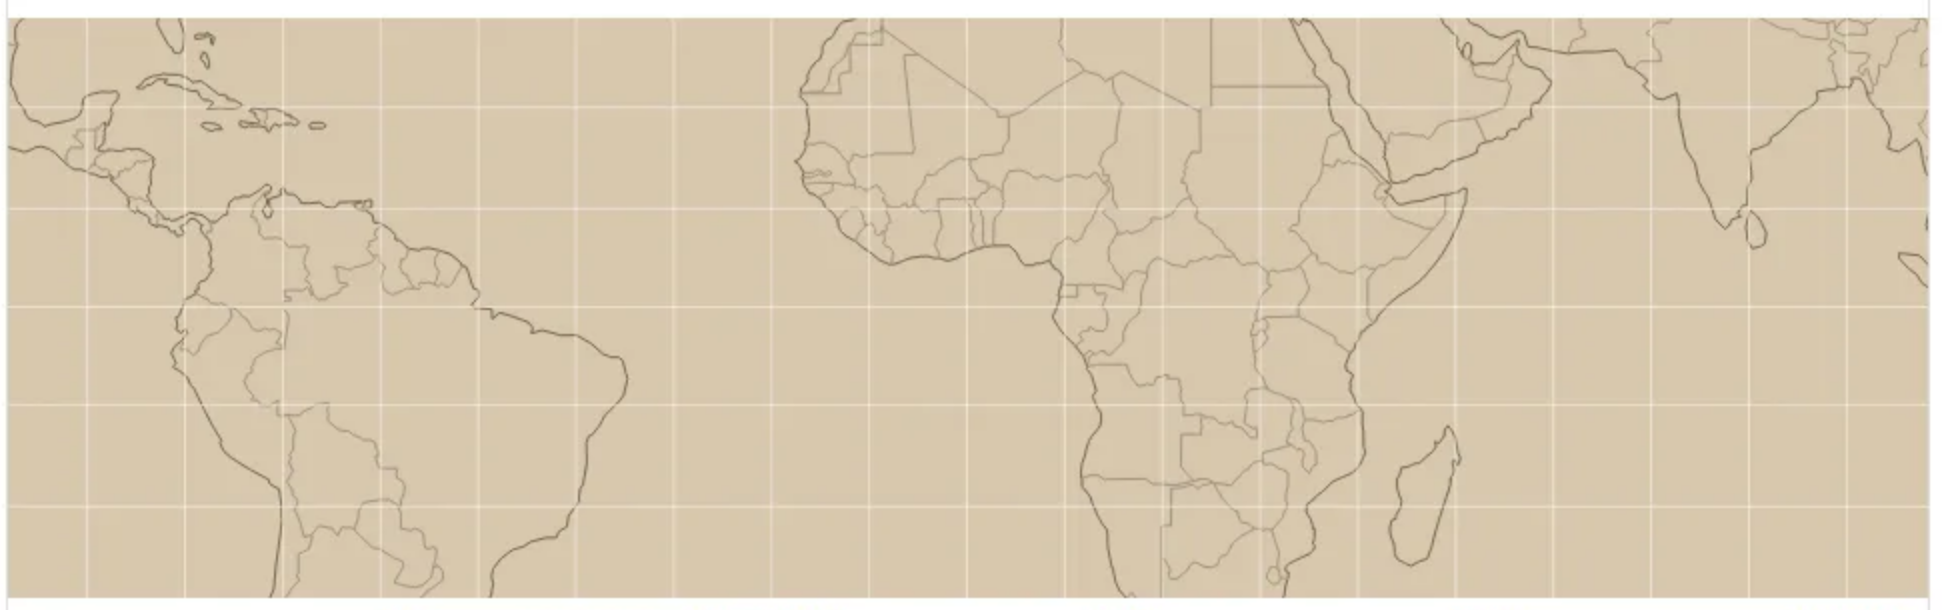
\includegraphics[scale=0.3]{figures/Mercator}
        \\
        \tiny
        Source: \url{https://www.geoawesomeness.com/all-map-projections-in-compared-and-visualized/}
 \end{figure}


\end{frame}
%----------------------------------------------------------------------%
\begin{frame}[fragile]
\frametitle{The earth ain't flat}
\framesubtitle{Mercator and the true size of countries}


\begin{figure}[H] \centering
            \captionsetup{justification=centering}
                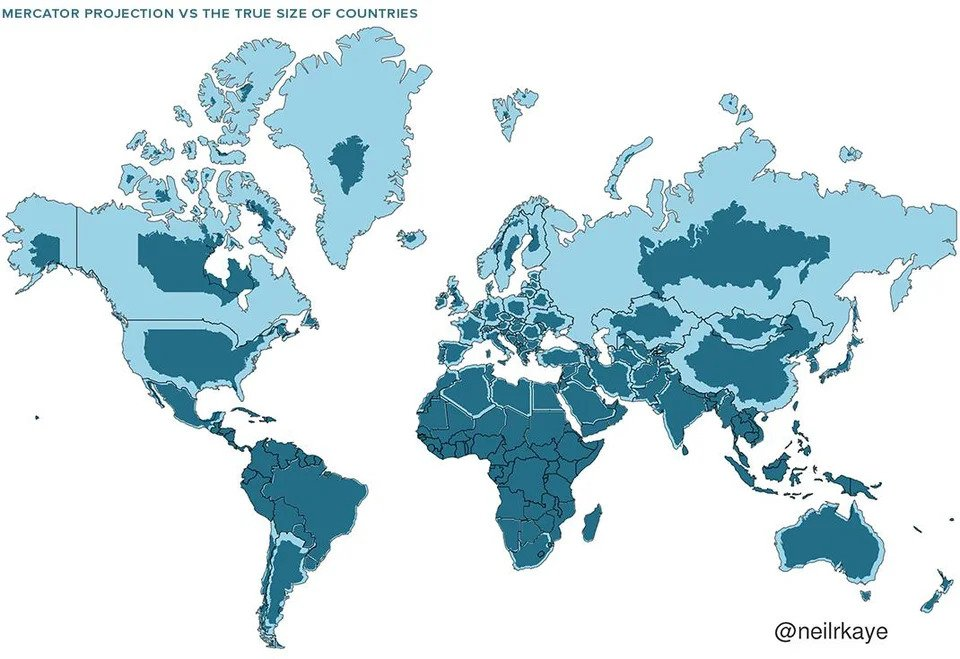
\includegraphics[scale=0.3]{figures/mercator_true_size.jpeg}
                \\
                \tiny
                Source: \url{https://www.reddit.com/r/Damnthatsinteresting/comments/xziol9/mercator_projection_vs_the_true_size_of_countries}
 \end{figure}


\end{frame}
%----------------------------------------------------------------------%
\begin{frame}[fragile]
\frametitle{Coordinate Reference System (CRS) }

\begin{itemize}
    \item With the help of coordinate reference systems (CRS) every place on the earth can be specified by  coordinates.
\end{itemize}


\begin{figure}[H] \centering
            \captionsetup{justification=centering}
                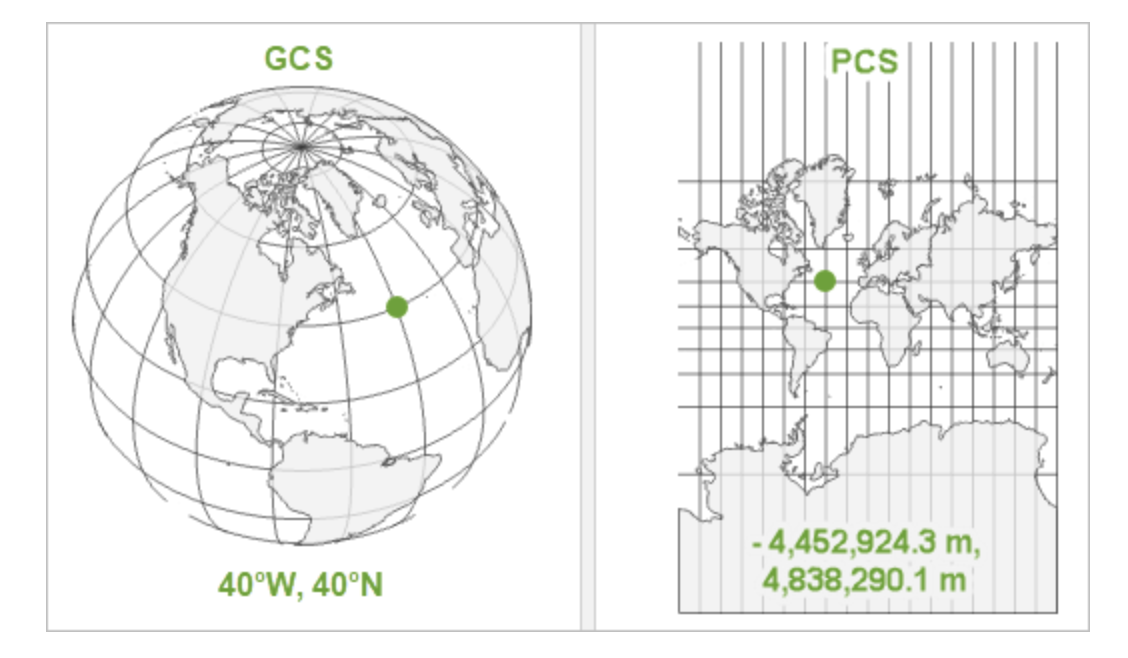
\includegraphics[scale=0.5]{figures/proj.png}
                \\
                \tiny
                Source: \url{https://www.geoawesomeness.com/all-map-projections-in-compared-and-visualized/}
 \end{figure}


\end{frame}

%----------------------------------------------------------------------%
\begin{frame}[fragile]
\frametitle{Which projection should I choose?}

\begin{itemize}

\item “There exist no all-purpose projections, all involve distortion when far from the center of the specified frame” (Bivand, Pebesma, and Gómez-Rubio 2013)
\medskip
\item The decision as to which map projection and coordinate reference system to use, depends on the regional extent of the area you want to work in, on the analysis you want to do and often on the availability of data.
\medskip
\item In some cases, it is not something that we are free to decide: “often the choice of projection is made by a public mapping agency” (Bivand, Pebesma, and Gómez-Rubio 2013).
\medskip
    \item  This means that when working with local data sources, it is likely preferable to work with the CRS in which the data was provided.
\end{itemize}

\end{frame}


%----------------------------------------------------------------------%
%----------------------------------------------------------------------%
\section{Spatial Dependence}
%----------------------------------------------------------------------%
%----------------------------------------------------------------------%

\begin{frame}[fragile]
\frametitle{Spatial Dependence}


    \begin{minipage}[t]{0.52\linewidth}
\bigskip
\begin{itemize}
  \small
   \item We now take a closer look at spatial dependence, or to be more precise on it's weaker expression spatial (auto)correlation. 
  \medskip

  \item Spatial autocorrelation measures the degree to which a phenomenon of interest is correlated to itself in space (Cliff and Ord (1973)). 
  \medskip
  \item For example, positive spatial correlation arises when units that are {\it close} to one another are more similar than units that are far apart
\end{itemize}

    \end{minipage}
    \hfill
    \begin{minipage}[t]{0.43\linewidth}%
       \medskip
        \begin{figure}[H] 
         
          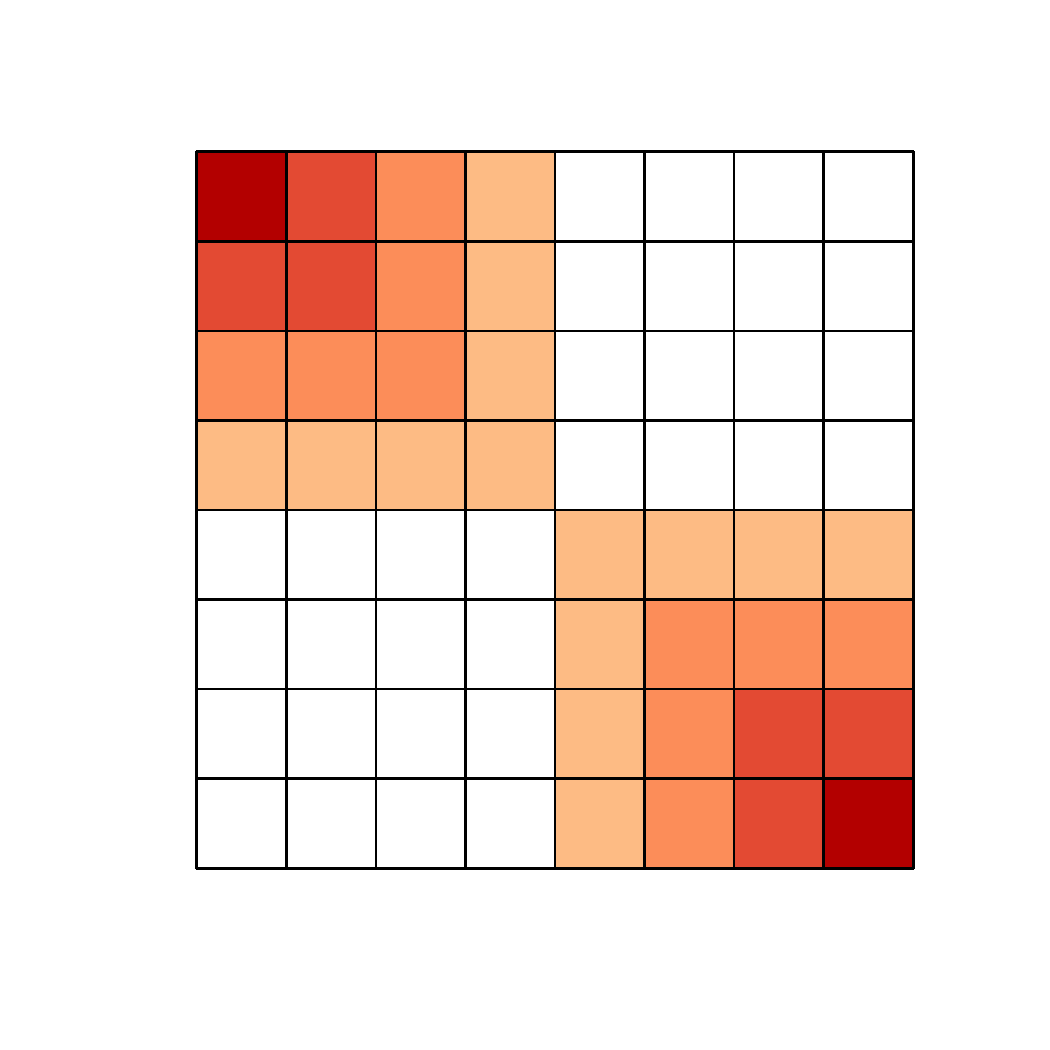
\includegraphics[scale=.35]{figures/spatial_correlation.pdf}
          
         

  \end{figure}
    \end{minipage}

\end{frame}
%----------------------------------------------------------------------%
\begin{frame}[fragile]
\frametitle{Spatial Dependence}

\begin{itemize}

  \medskip
  \item  We can express the existence of spatial autocorrelation with the following moment condition:
\medskip


\begin{equation}
 Cov(y_{i},y_{j})\neq 0\,\,\,\,for\,\,\,\,i\neq j
\end{equation}

were \(y_i\) and \(y_j\) are observations on a random variable at locations \(i\) and \(j\). 
\medskip
  \item This autocorrelation can lead to overfitting of the model and poor generalization to new spatial locations. 
  \medskip
  \item By using spatial cross-validation, we can ensure that the model is tested on data that is independent of the training data and has similar spatial characteristics.
\end{itemize}

\end{frame}
%----------------------------------------------------------------------%
\begin{frame}[fragile]
\frametitle{Spatial Prediction}

\begin{figure}[H] \centering
            \captionsetup{justification=centering}
    
\includegraphics[scale=0.4]{figures/spatial_cross/fig01.png}
\\
\tiny
Source: \url{https://www.youtube.com/watch?v=TK_2MIbChb0&ab_channel=CAUSEweb}
 \end{figure}
\end{frame}
%----------------------------------------------------------------------%
\begin{frame}[fragile]
\frametitle{Spatial Prediction}

\begin{figure}[H] \centering
            \captionsetup{justification=centering}
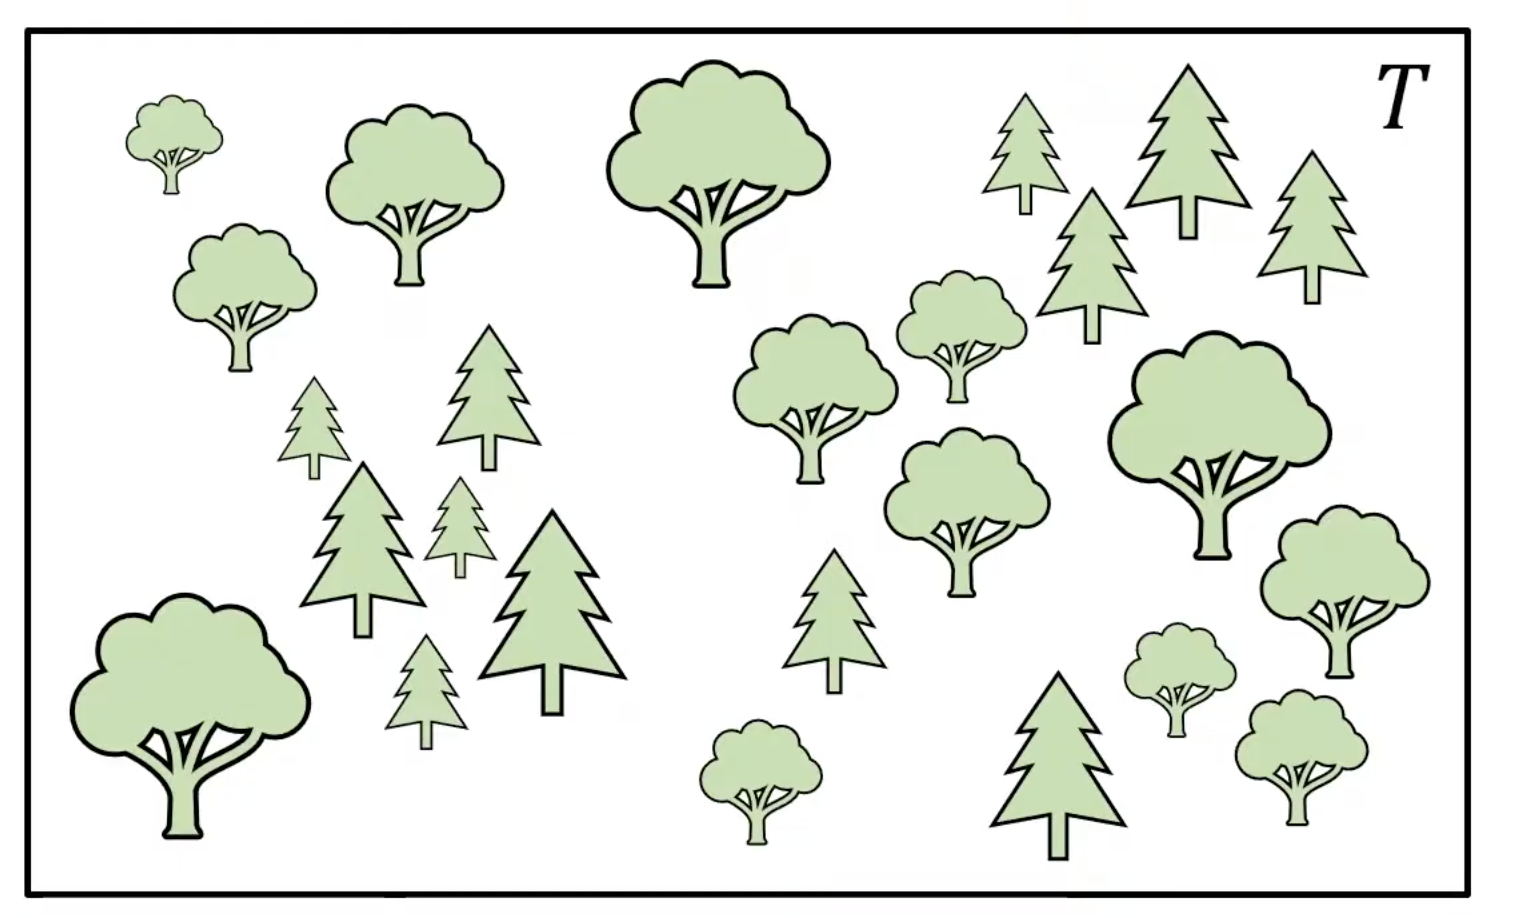
\includegraphics[scale=0.4]{figures/spatial_cross/fig02.png}
\\
\tiny
Source: \url{https://www.youtube.com/watch?v=TK_2MIbChb0&ab_channel=CAUSEweb}
 \end{figure}
\end{frame}
%----------------------------------------------------------------------%

\begin{frame}[fragile]
\frametitle{Spatial Prediction}

\begin{figure}[H] \centering
            \captionsetup{justification=centering}
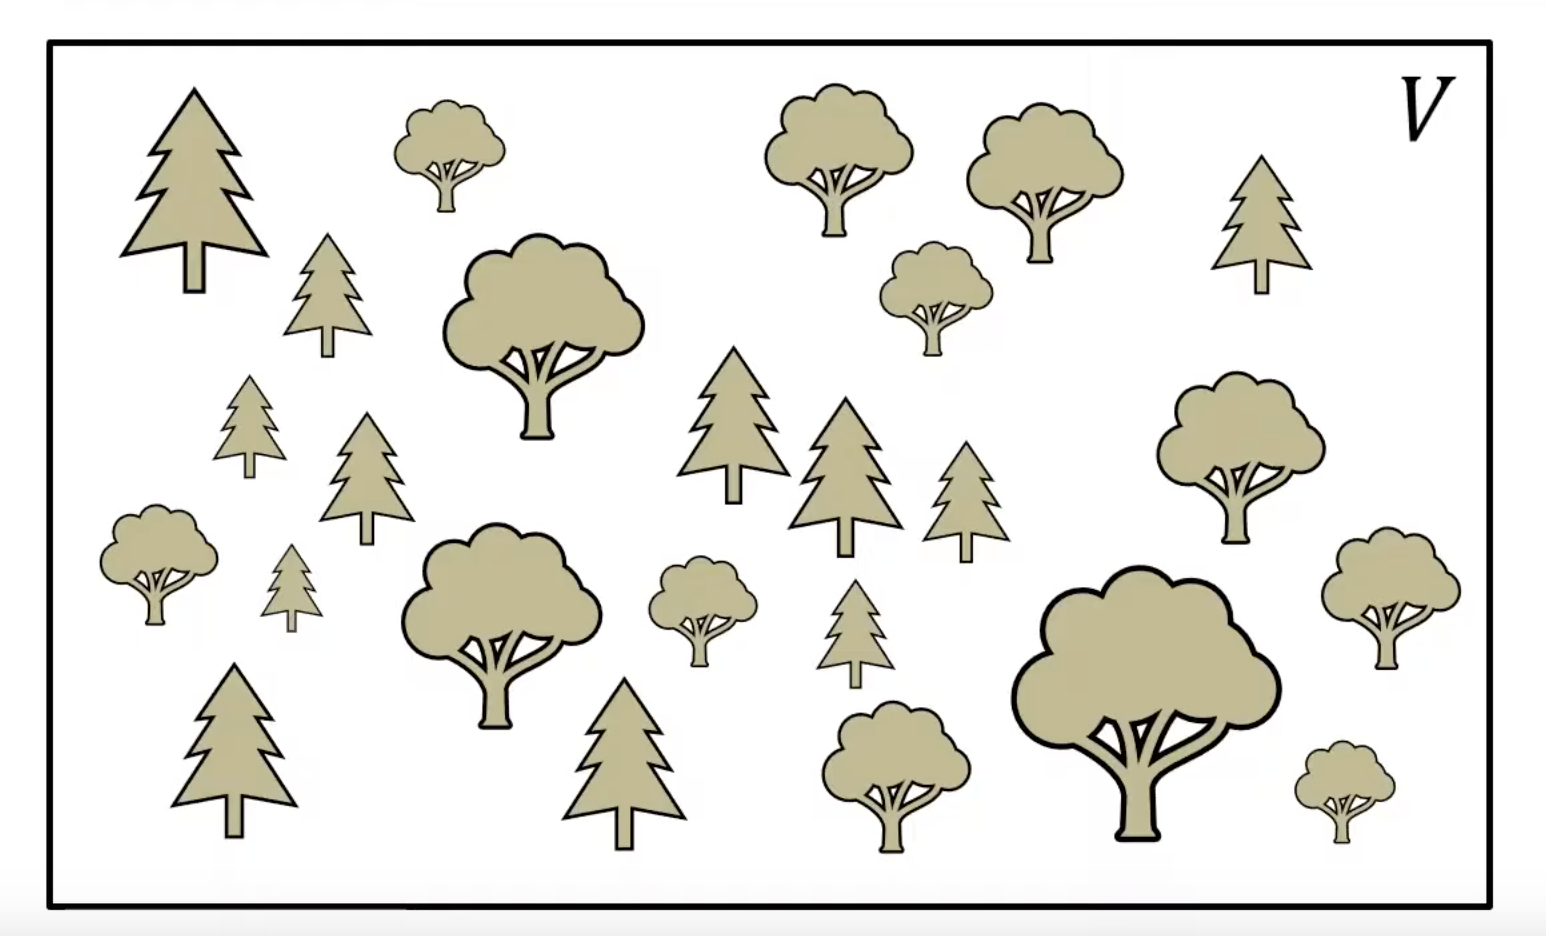
\includegraphics[scale=0.4]{figures/spatial_cross/fig03.png}
\\
\tiny
Source: \url{https://www.youtube.com/watch?v=TK_2MIbChb0&ab_channel=CAUSEweb}
 \end{figure}
\end{frame}
%----------------------------------------------------------------------%

\begin{frame}[fragile]
\frametitle{Spatial Prediction}

\begin{figure}[H] \centering
            \captionsetup{justification=centering}
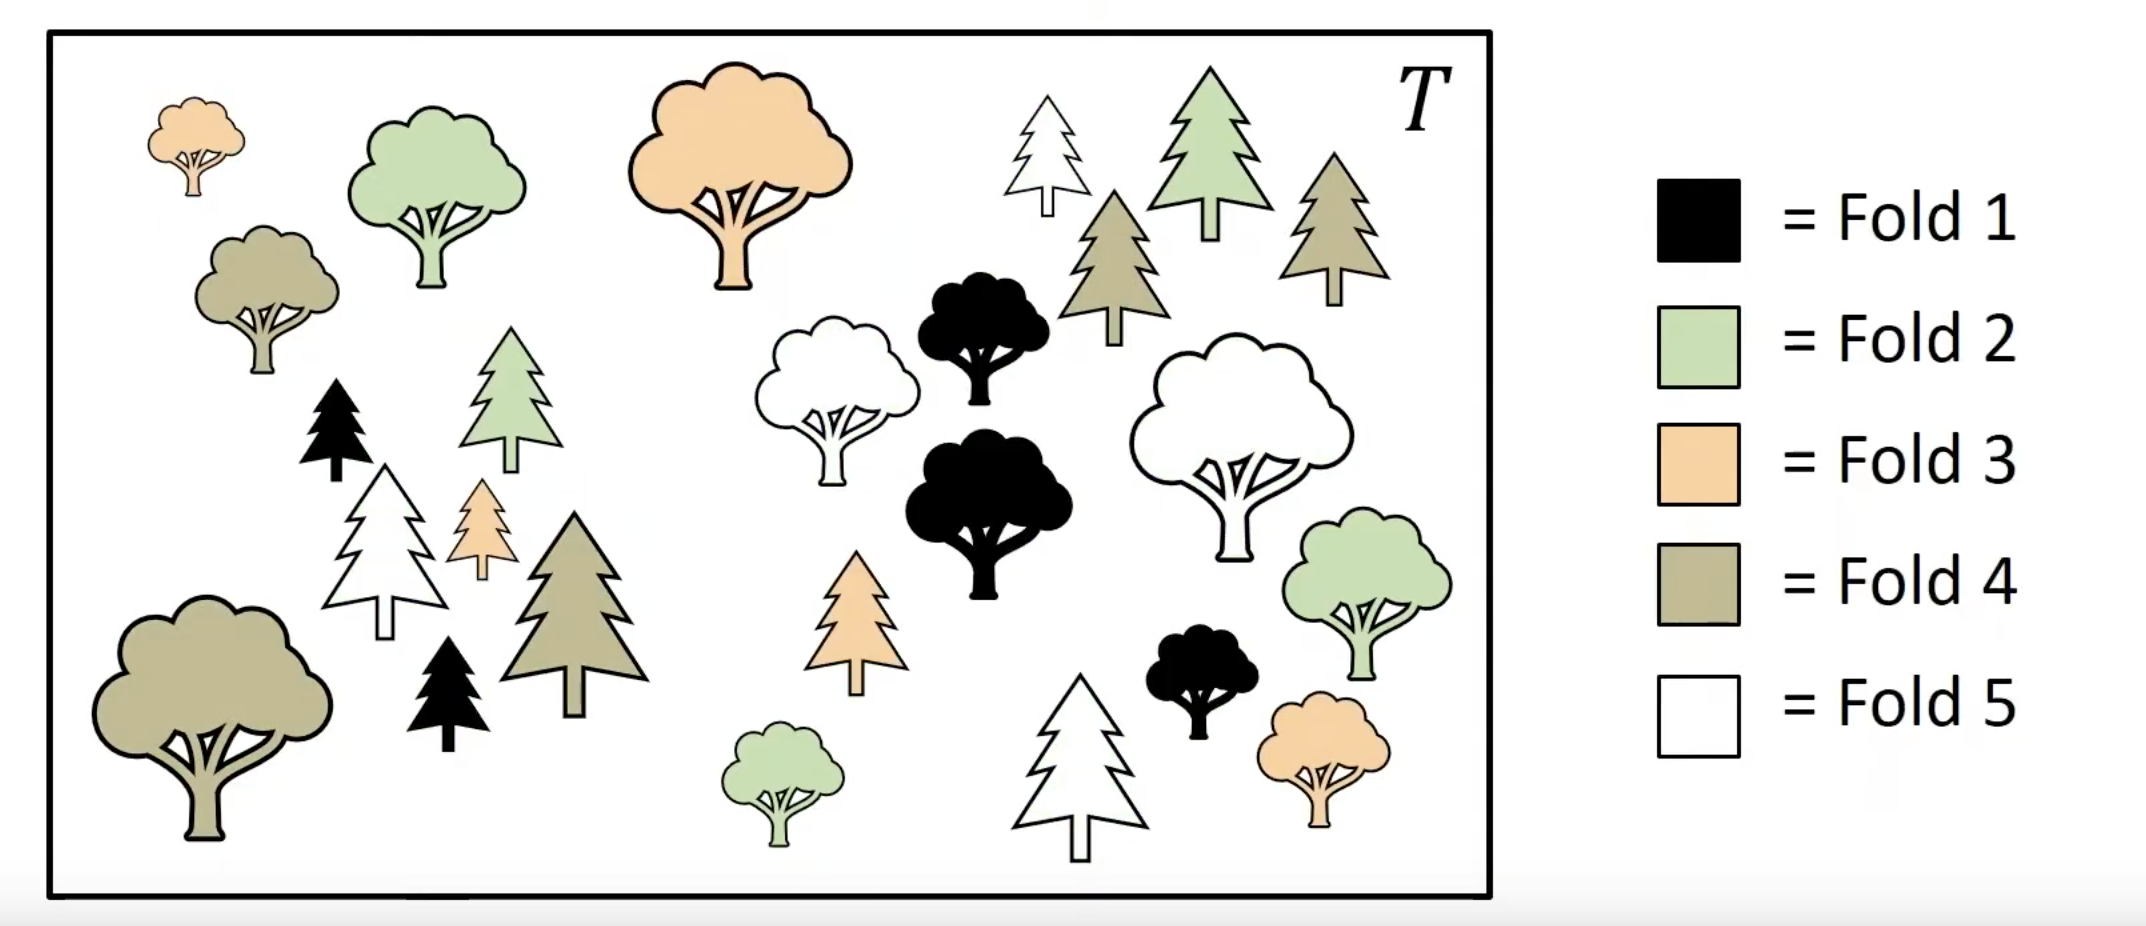
\includegraphics[scale=0.3]{figures/spatial_cross/fig04.png}
\\
\tiny
Source: \url{https://www.youtube.com/watch?v=TK_2MIbChb0&ab_channel=CAUSEweb}
 \end{figure}
\end{frame}
%----------------------------------------------------------------------%

\begin{frame}[fragile]
\frametitle{Spatial Prediction}

\begin{figure}[H] \centering
            \captionsetup{justification=centering}
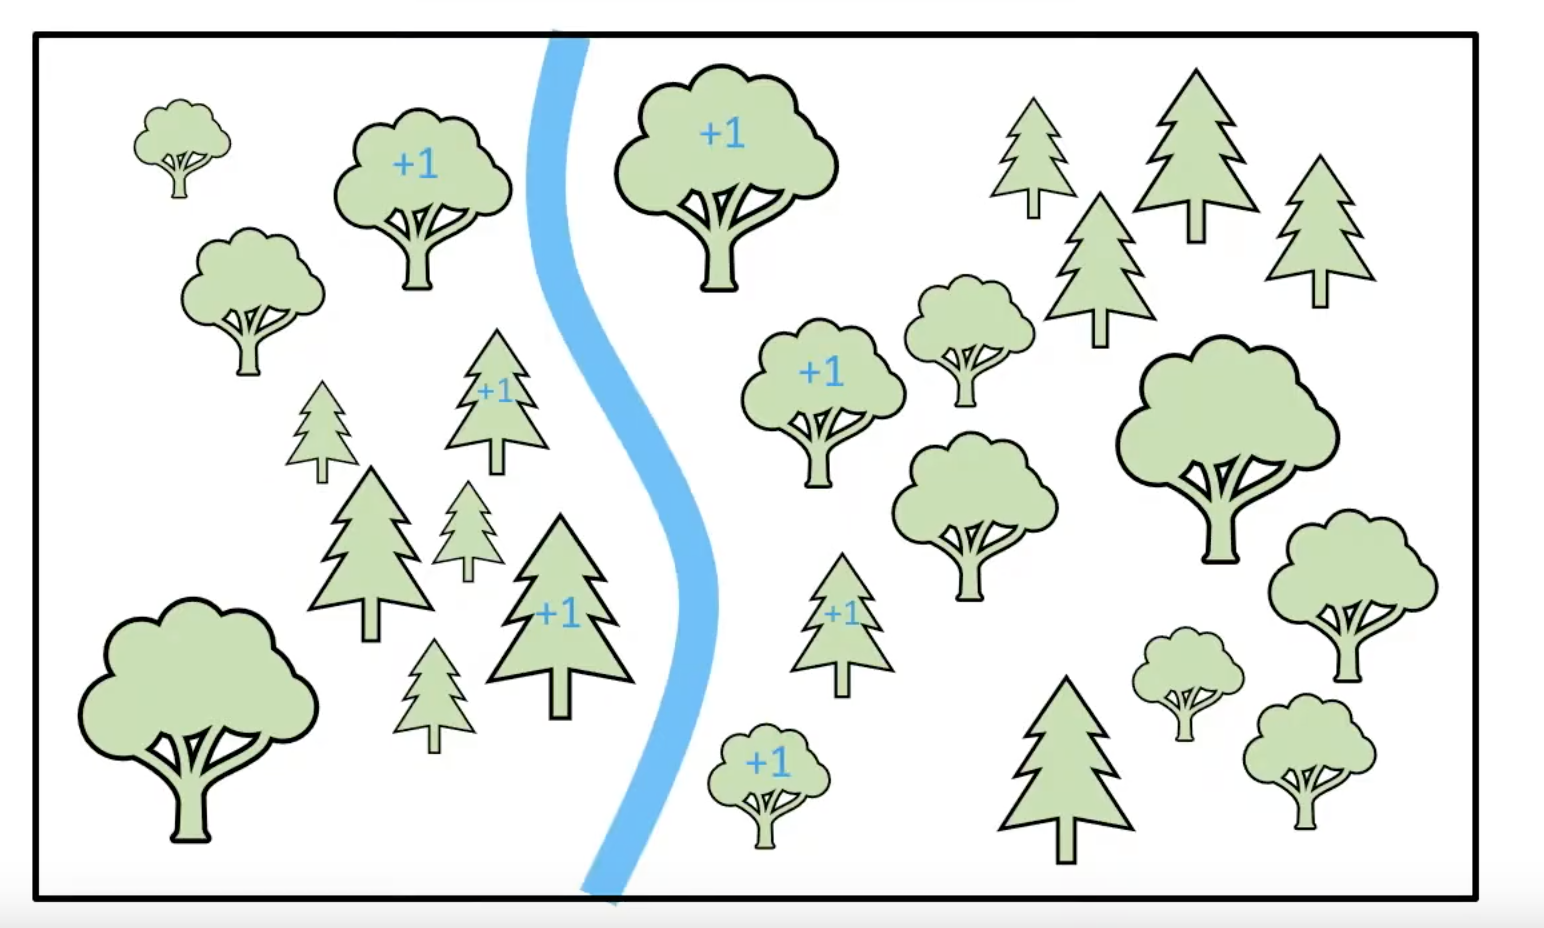
\includegraphics[scale=0.4]{figures/spatial_cross/fig05.png}
\\
\tiny
Source: \url{https://www.youtube.com/watch?v=TK_2MIbChb0&ab_channel=CAUSEweb}
 \end{figure}
\end{frame}
%----------------------------------------------------------------------%

\begin{frame}[fragile]
\frametitle{Spatial Prediction}

\begin{figure}[H] \centering
            \captionsetup{justification=centering}
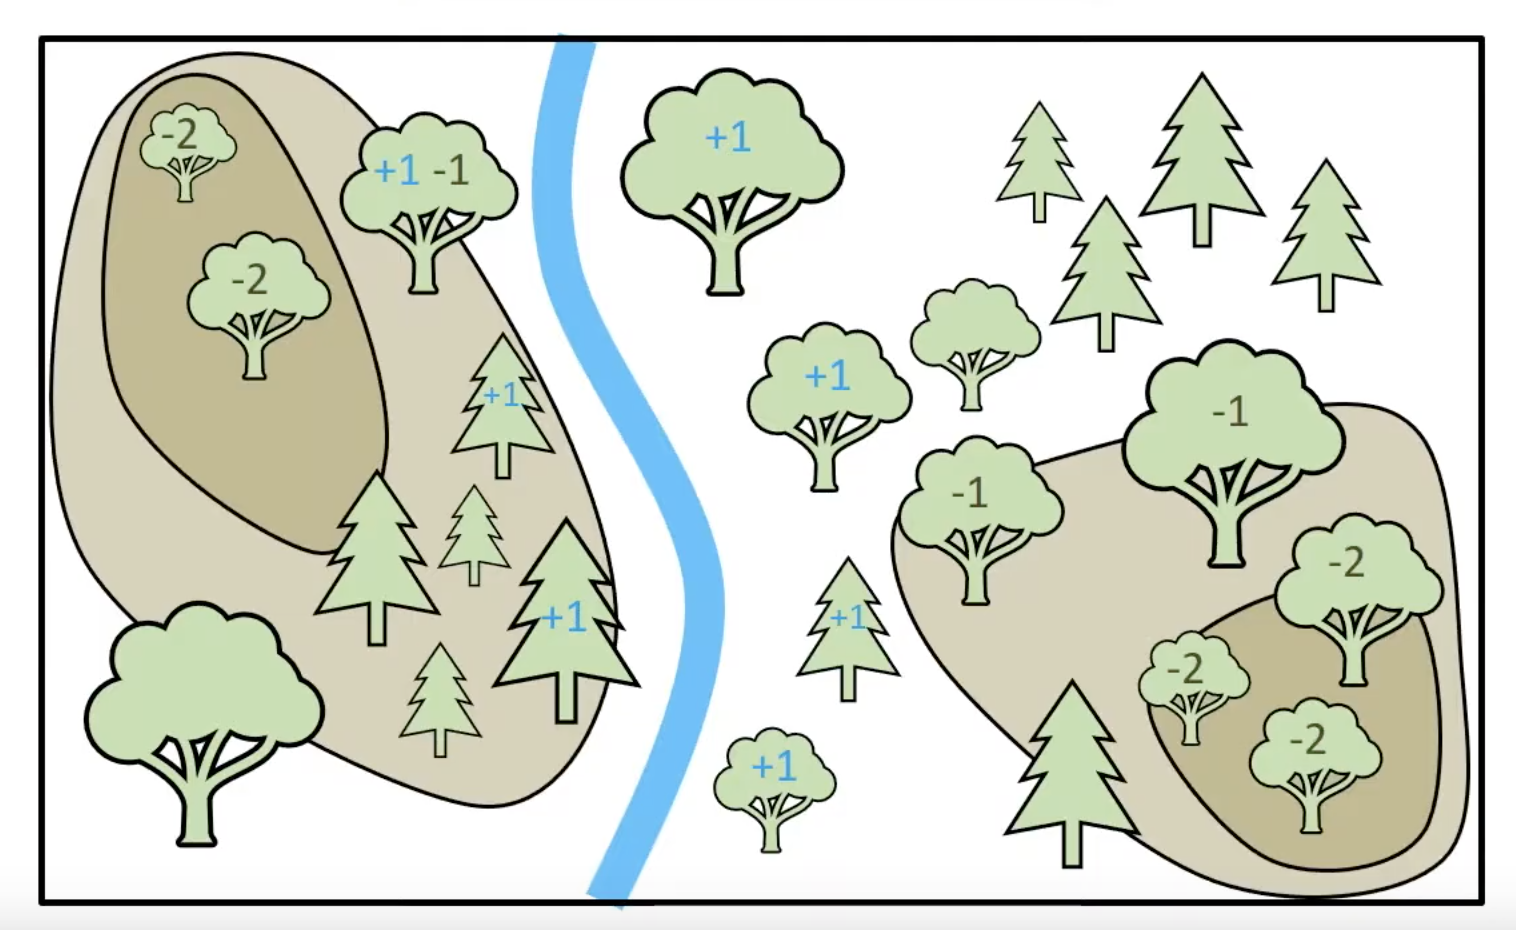
\includegraphics[scale=0.4]{figures/spatial_cross/fig06.png}
\\
\tiny
Source: \url{https://www.youtube.com/watch?v=TK_2MIbChb0&ab_channel=CAUSEweb}
 \end{figure}
\end{frame}
%----------------------------------------------------------------------%

\begin{frame}[fragile]
\frametitle{Spatial Prediction}

\begin{figure}[H] \centering
            \captionsetup{justification=centering}
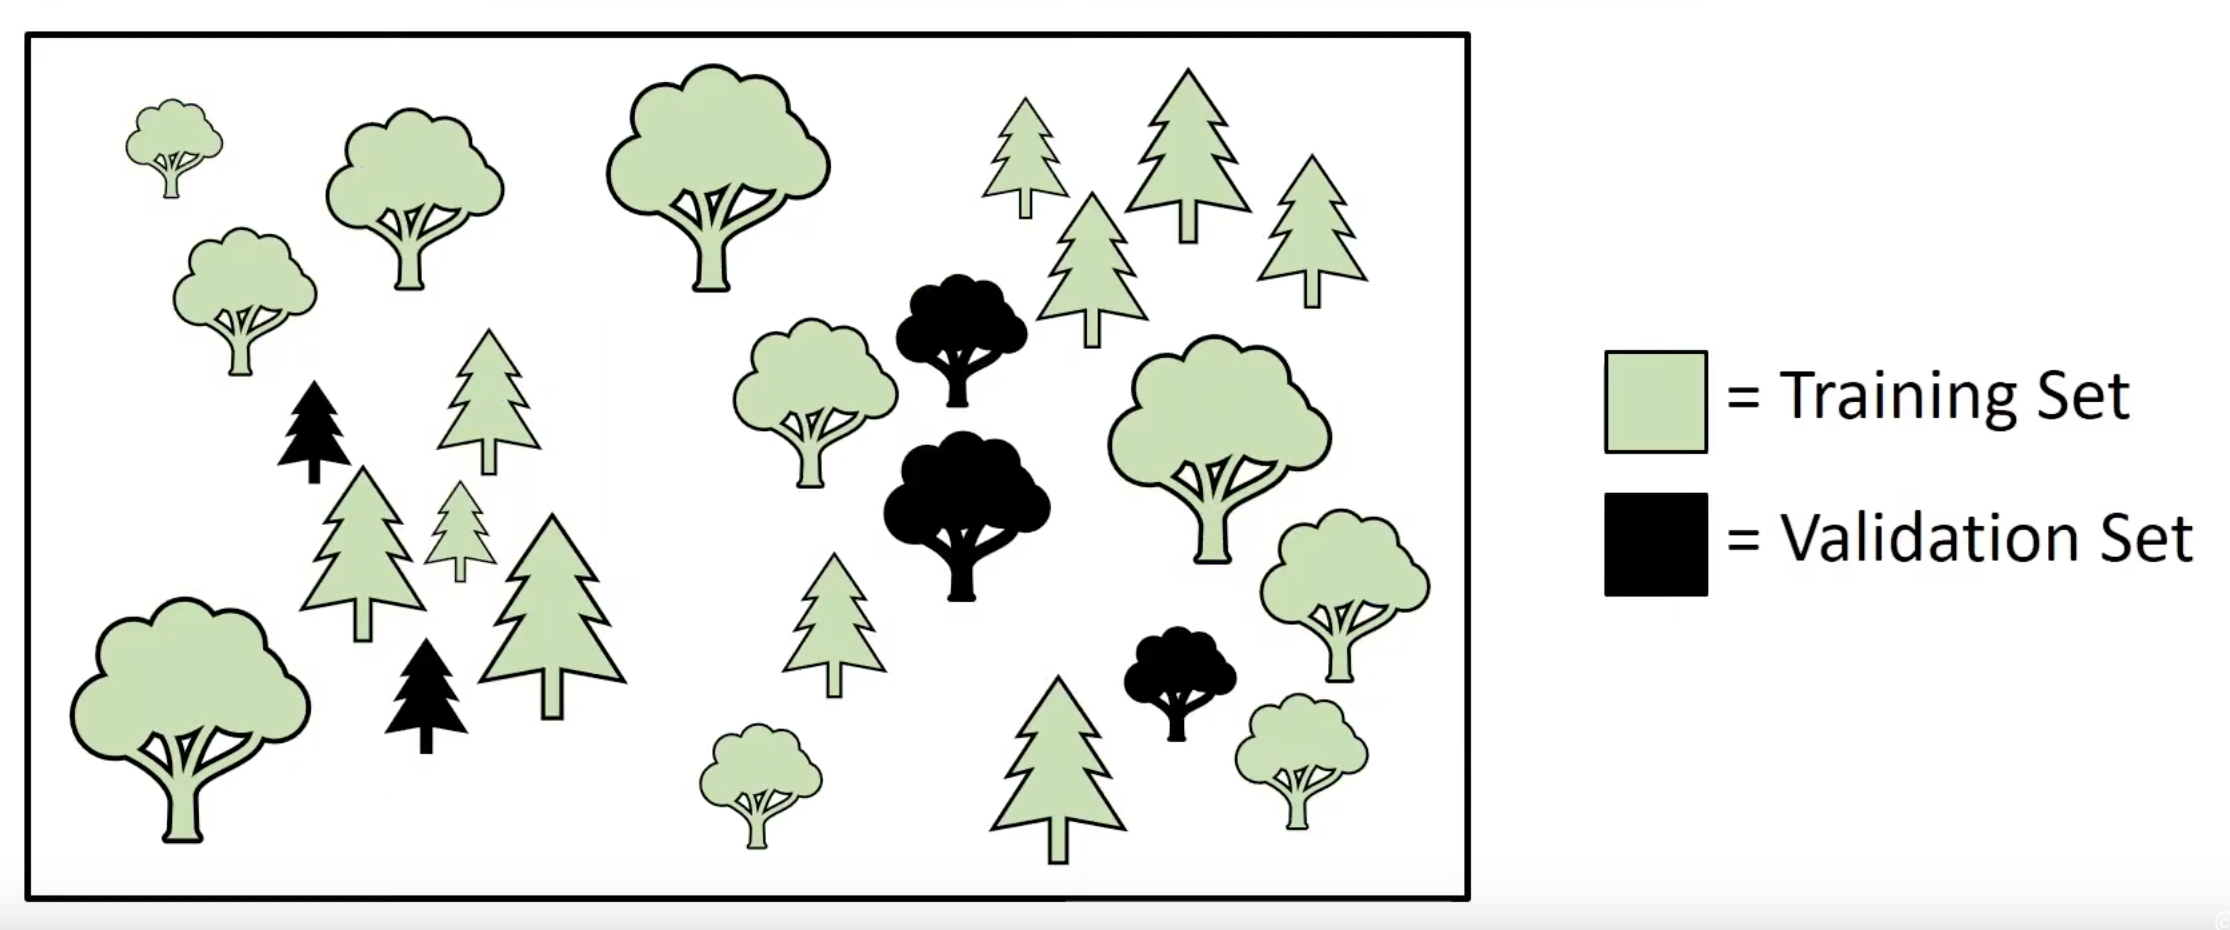
\includegraphics[scale=0.3]{figures/spatial_cross/fig07.png}
\\
\tiny
Source: \url{https://www.youtube.com/watch?v=TK_2MIbChb0&ab_channel=CAUSEweb}
 \end{figure}
\end{frame}
%----------------------------------------------------------------------%

\begin{frame}[fragile]
\frametitle{Spatial Prediction}

\begin{figure}[H] \centering
            \captionsetup{justification=centering}
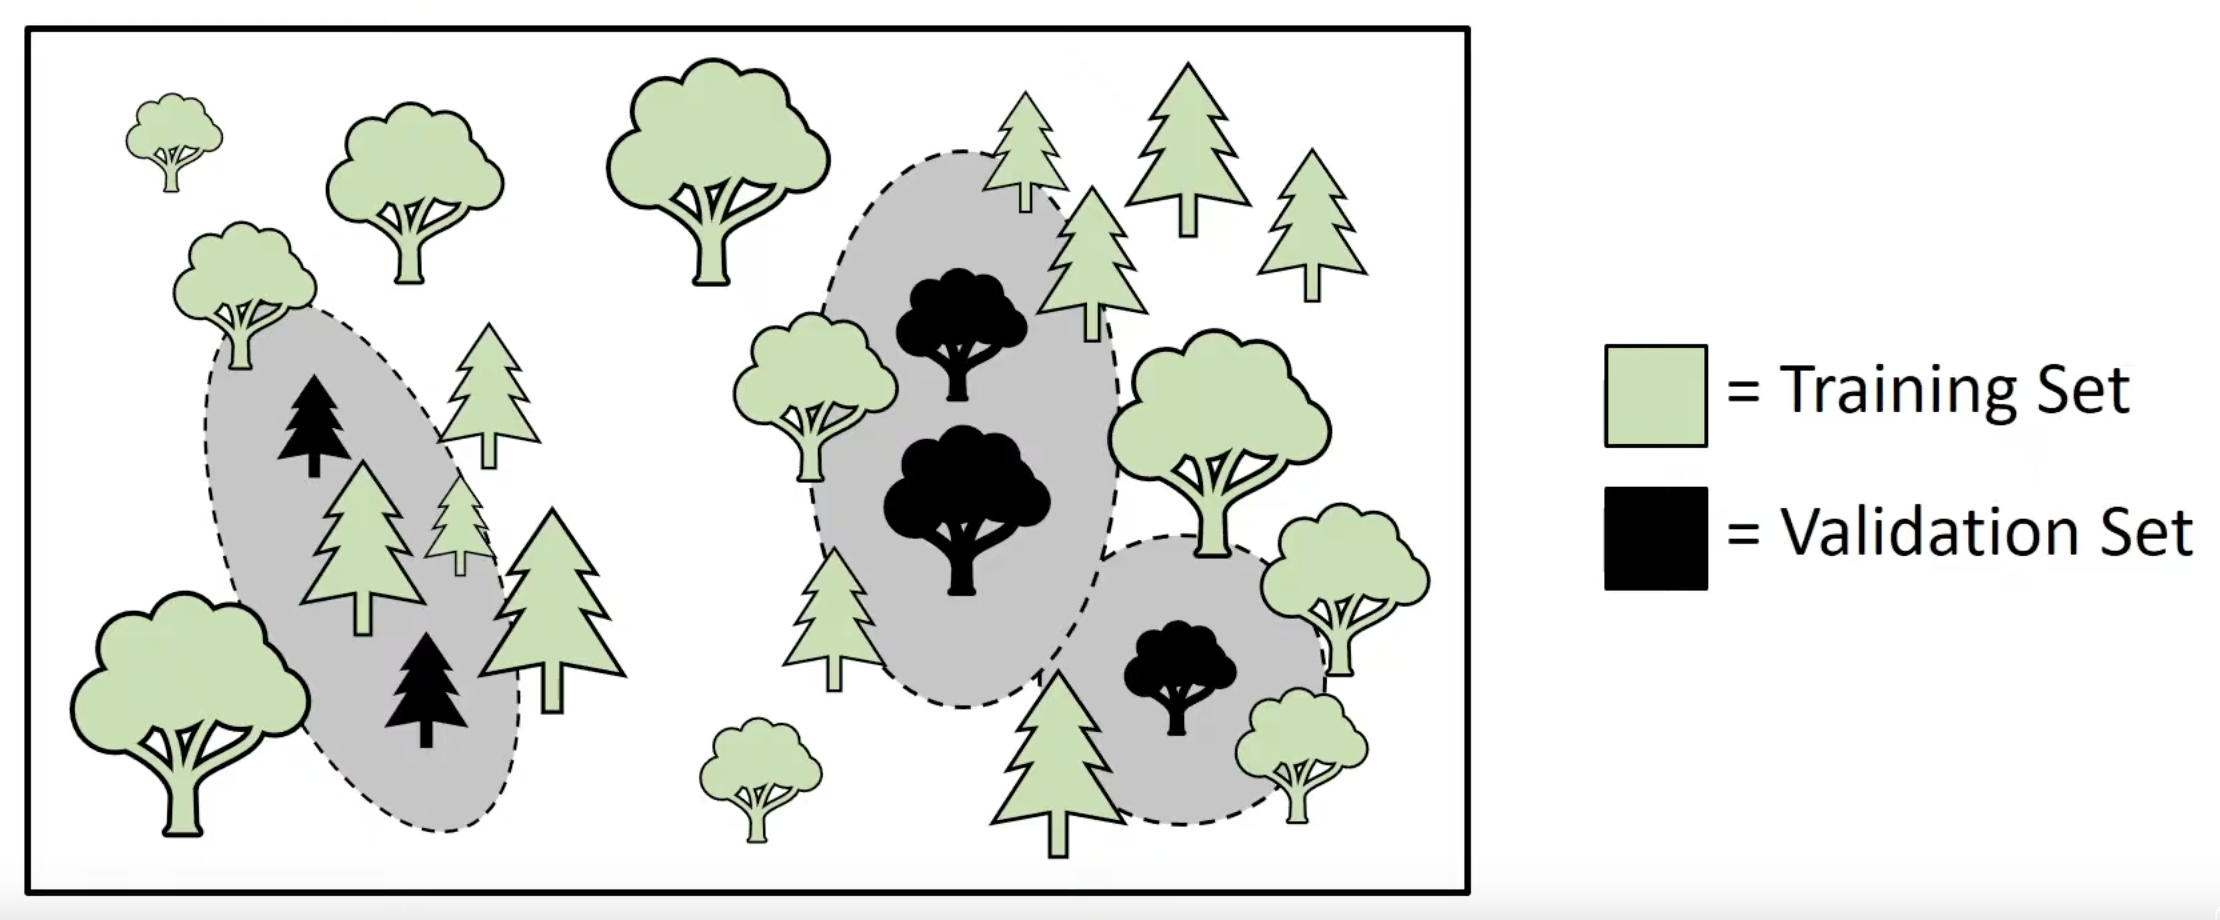
\includegraphics[scale=0.3]{figures/spatial_cross/fig08.png}
\\
\tiny
Source: \url{https://www.youtube.com/watch?v=TK_2MIbChb0&ab_channel=CAUSEweb}
 \end{figure}
\end{frame}
%----------------------------------------------------------------------%

\begin{frame}[fragile]
\frametitle{Spatial Prediction}

\begin{figure}[H] \centering
            \captionsetup{justification=centering}
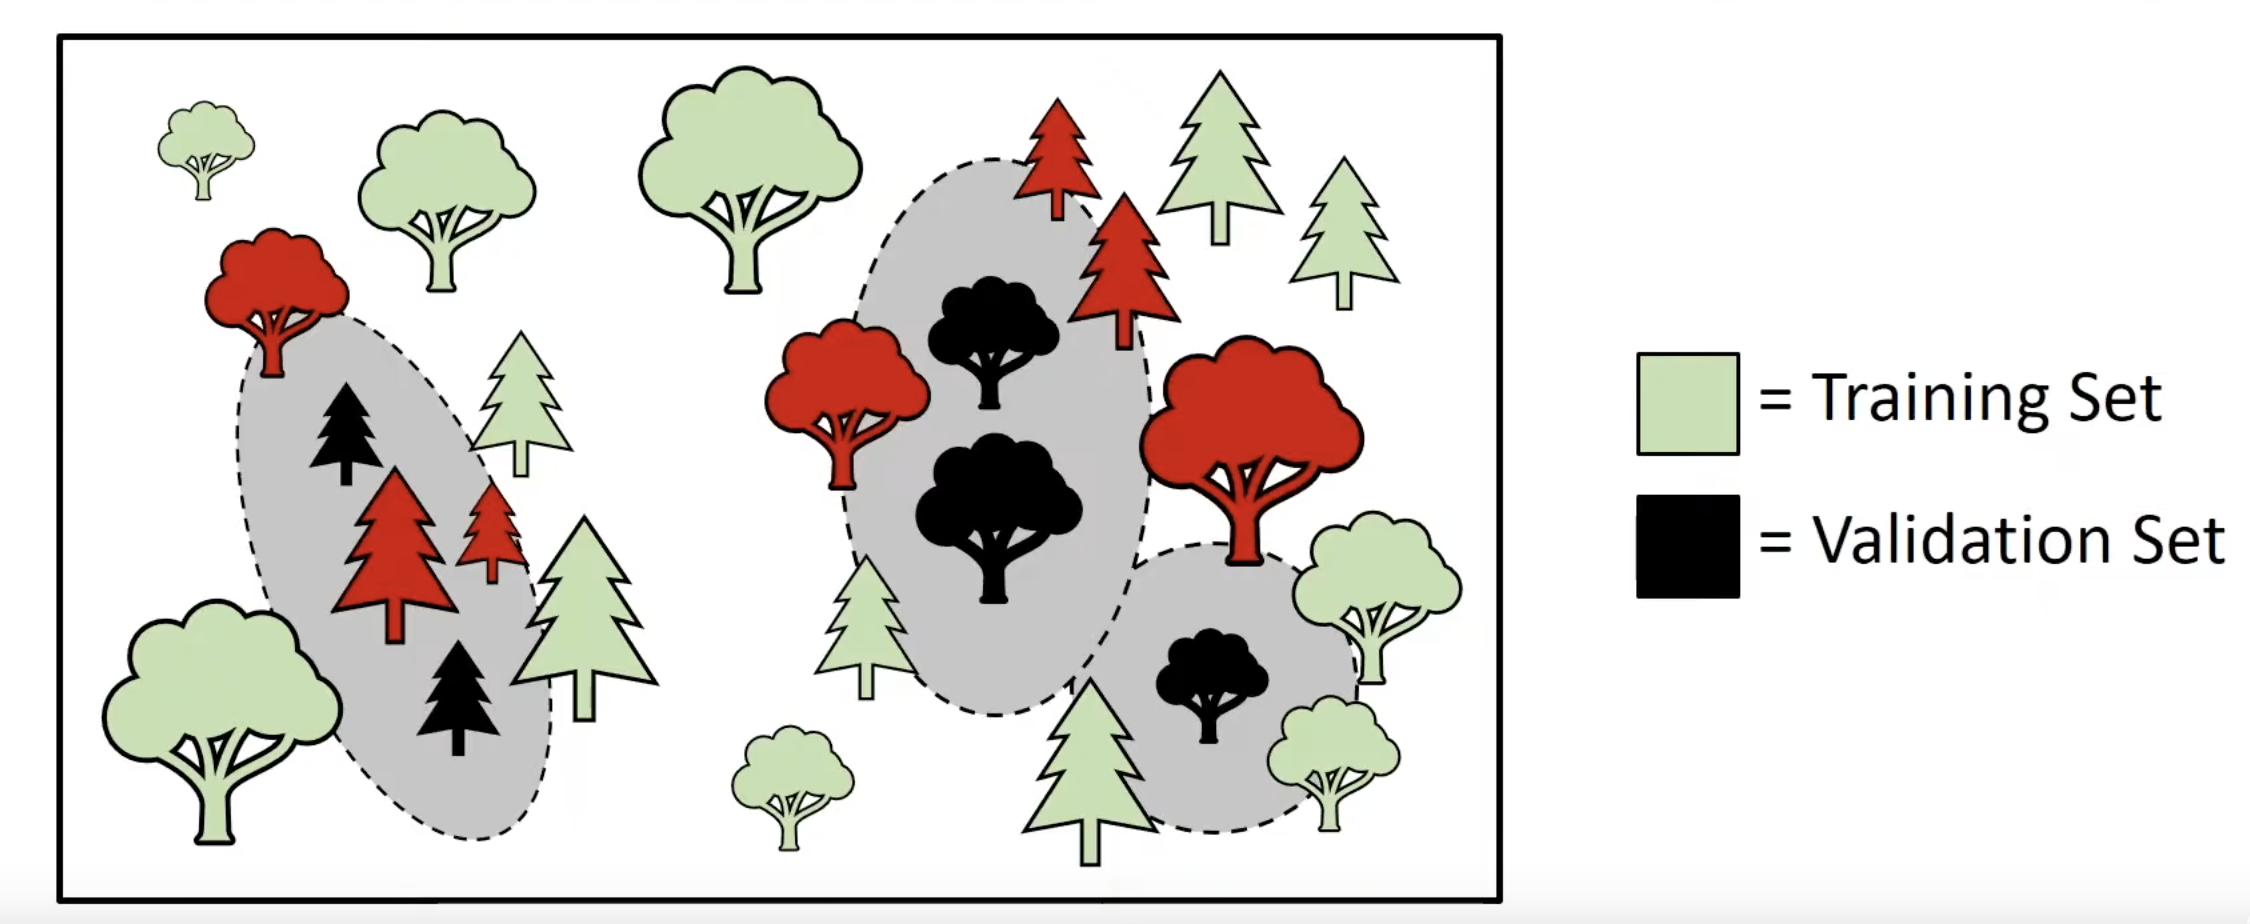
\includegraphics[scale=0.3]{figures/spatial_cross/fig09.png}
\\
\tiny
Source: \url{https://www.youtube.com/watch?v=TK_2MIbChb0&ab_channel=CAUSEweb}
 \end{figure}
\end{frame}
%----------------------------------------------------------------------%

\begin{frame}[fragile]
\frametitle{Spatial Prediction}

\begin{figure}[H] \centering
            \captionsetup{justification=centering}
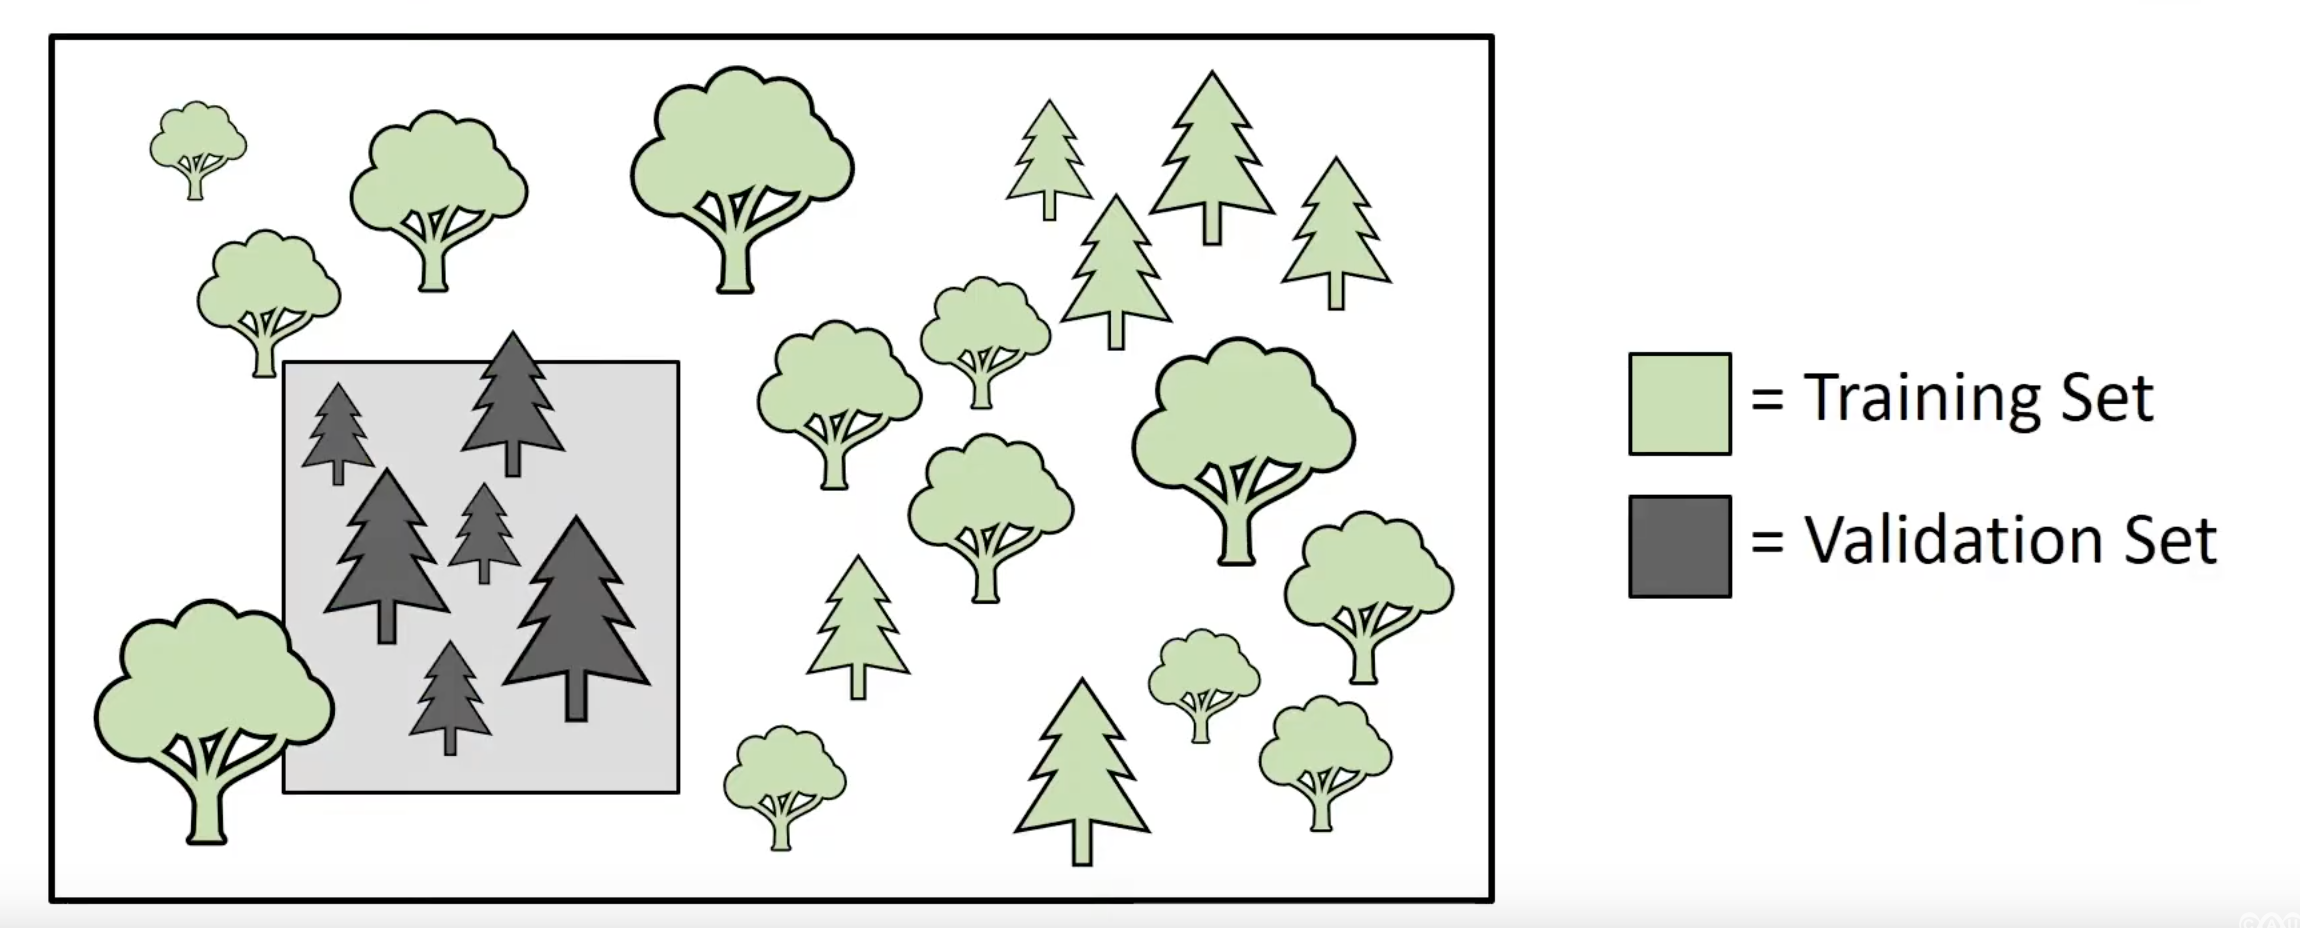
\includegraphics[scale=0.3]{figures/spatial_cross/fig10.png}
\\
\tiny
Source: \url{https://www.youtube.com/watch?v=TK_2MIbChb0&ab_channel=CAUSEweb}
 \end{figure}
\end{frame}
%----------------------------------------------------------------------%

\begin{frame}[fragile]
\frametitle{Spatial Prediction}

\begin{figure}[H] \centering
            \captionsetup{justification=centering}
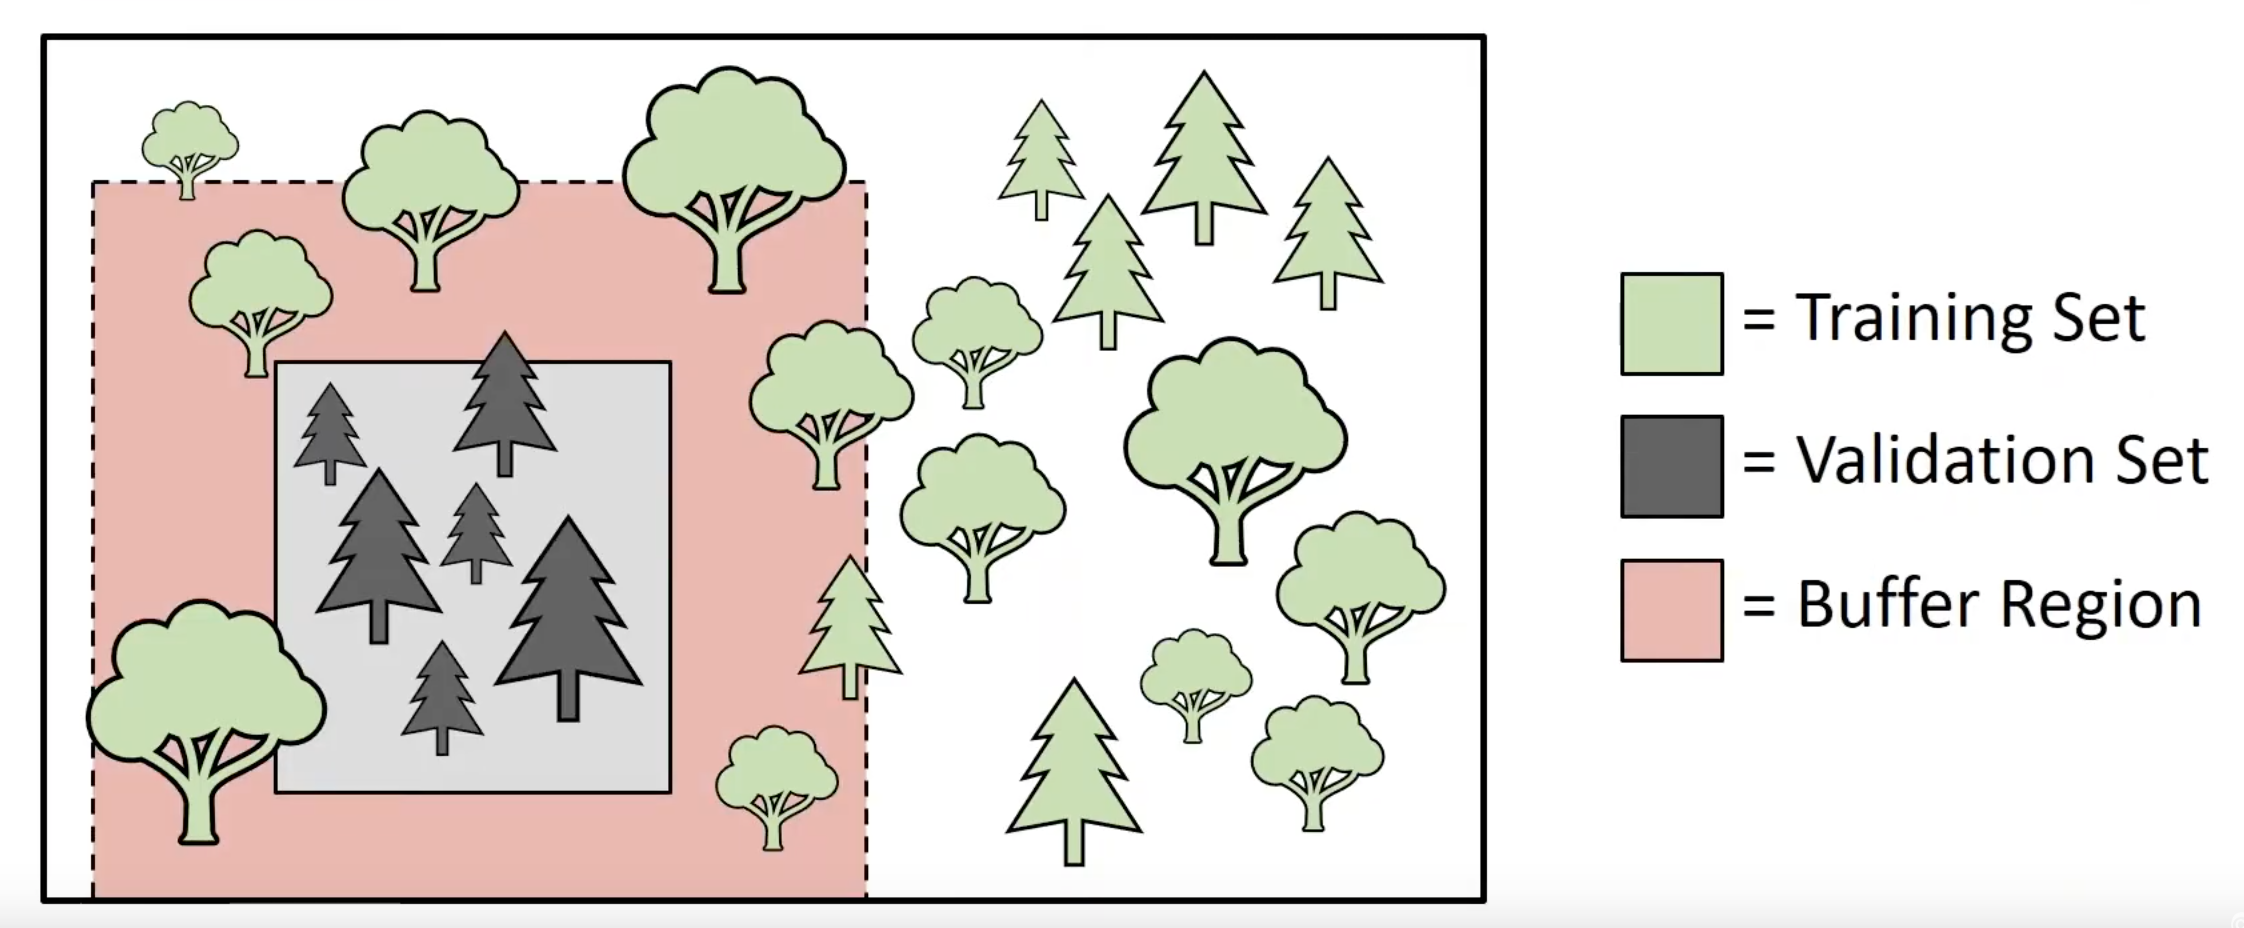
\includegraphics[scale=0.3]{figures/spatial_cross/fig11.png}
\\
\tiny
Source: \url{https://www.youtube.com/watch?v=TK_2MIbChb0&ab_channel=CAUSEweb}
 \end{figure}
\end{frame}
%----------------------------------------------------------------------%

\begin{frame}[fragile]
\frametitle{Spatial Prediction}

\begin{figure}[H] \centering
            \captionsetup{justification=centering}
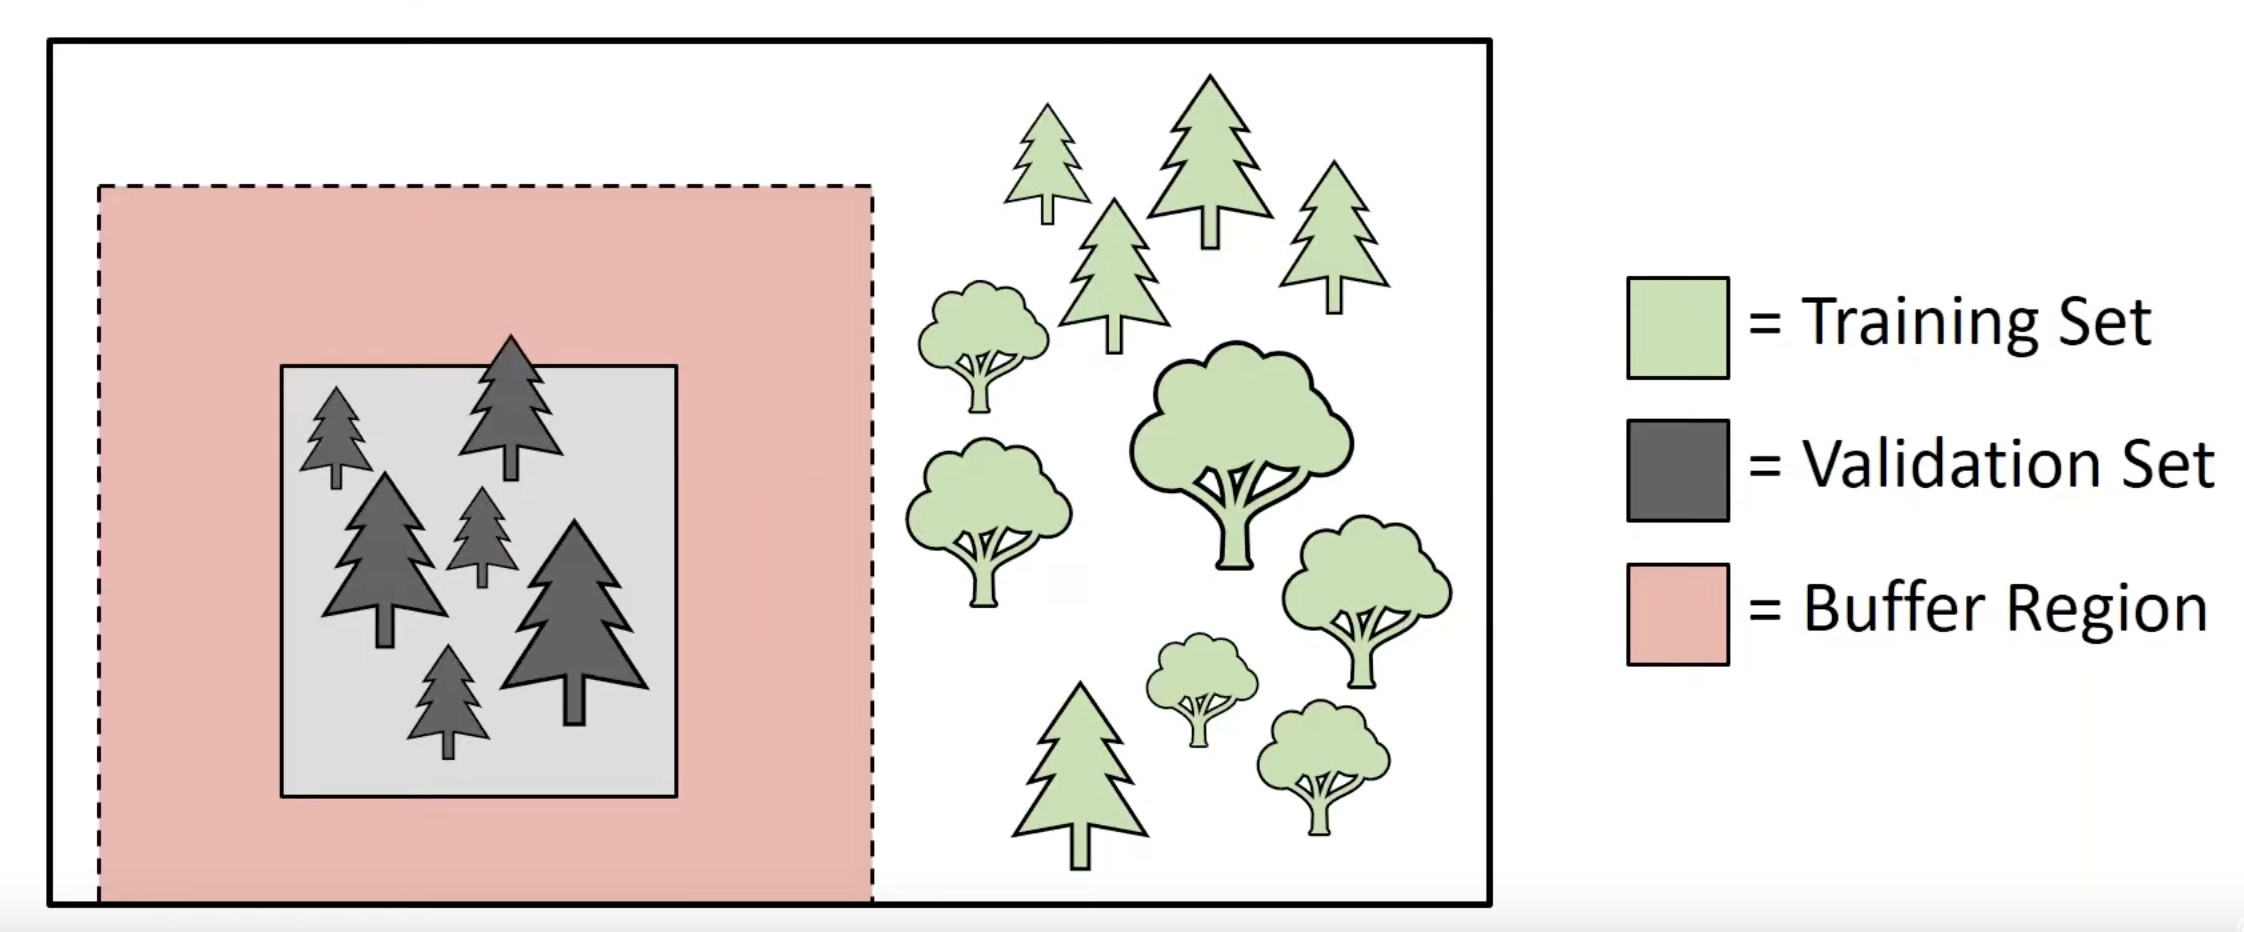
\includegraphics[scale=0.3]{figures/spatial_cross/fig12.png}
\\
\tiny
Source: \url{https://www.youtube.com/watch?v=TK_2MIbChb0&ab_channel=CAUSEweb}
 \end{figure}
\end{frame}
%----------------------------------------------------------------------%

\begin{frame}[fragile]
\frametitle{Spatial Prediction}

\begin{figure}[H] \centering
            \captionsetup{justification=centering}
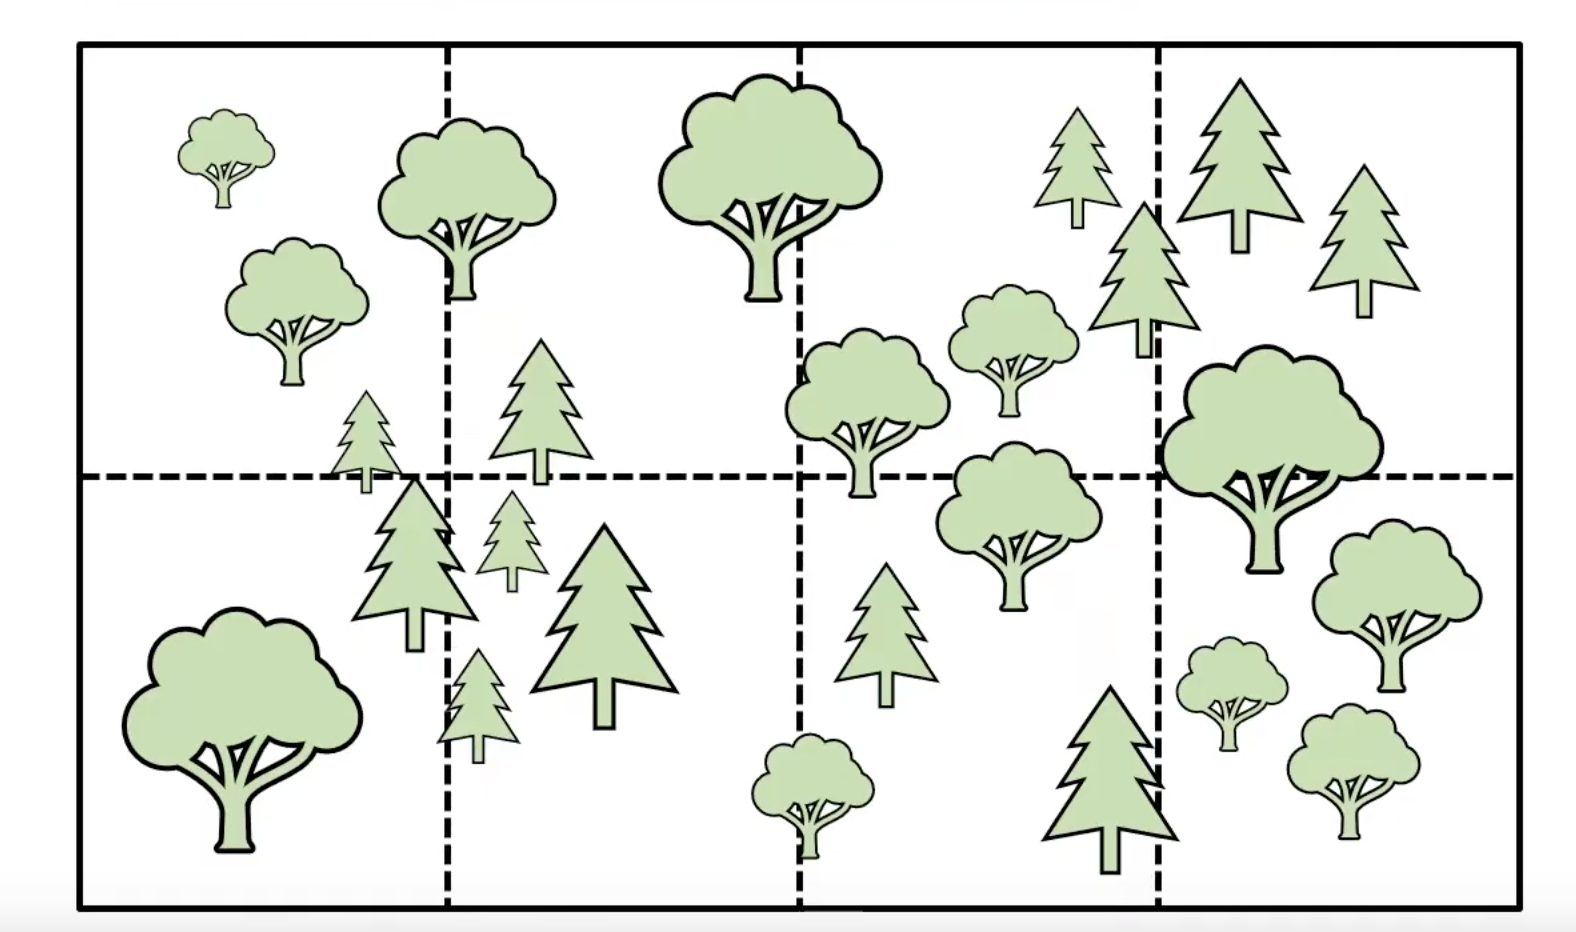
\includegraphics[scale=0.4]{figures/spatial_cross/fig13.png}
\\
\tiny
Source: \url{https://www.youtube.com/watch?v=TK_2MIbChb0&ab_channel=CAUSEweb}
 \end{figure}
\end{frame}
%----------------------------------------------------------------------%

\begin{frame}[fragile]
\frametitle{Spatial Prediction}

\begin{figure}[H] \centering
            \captionsetup{justification=centering}
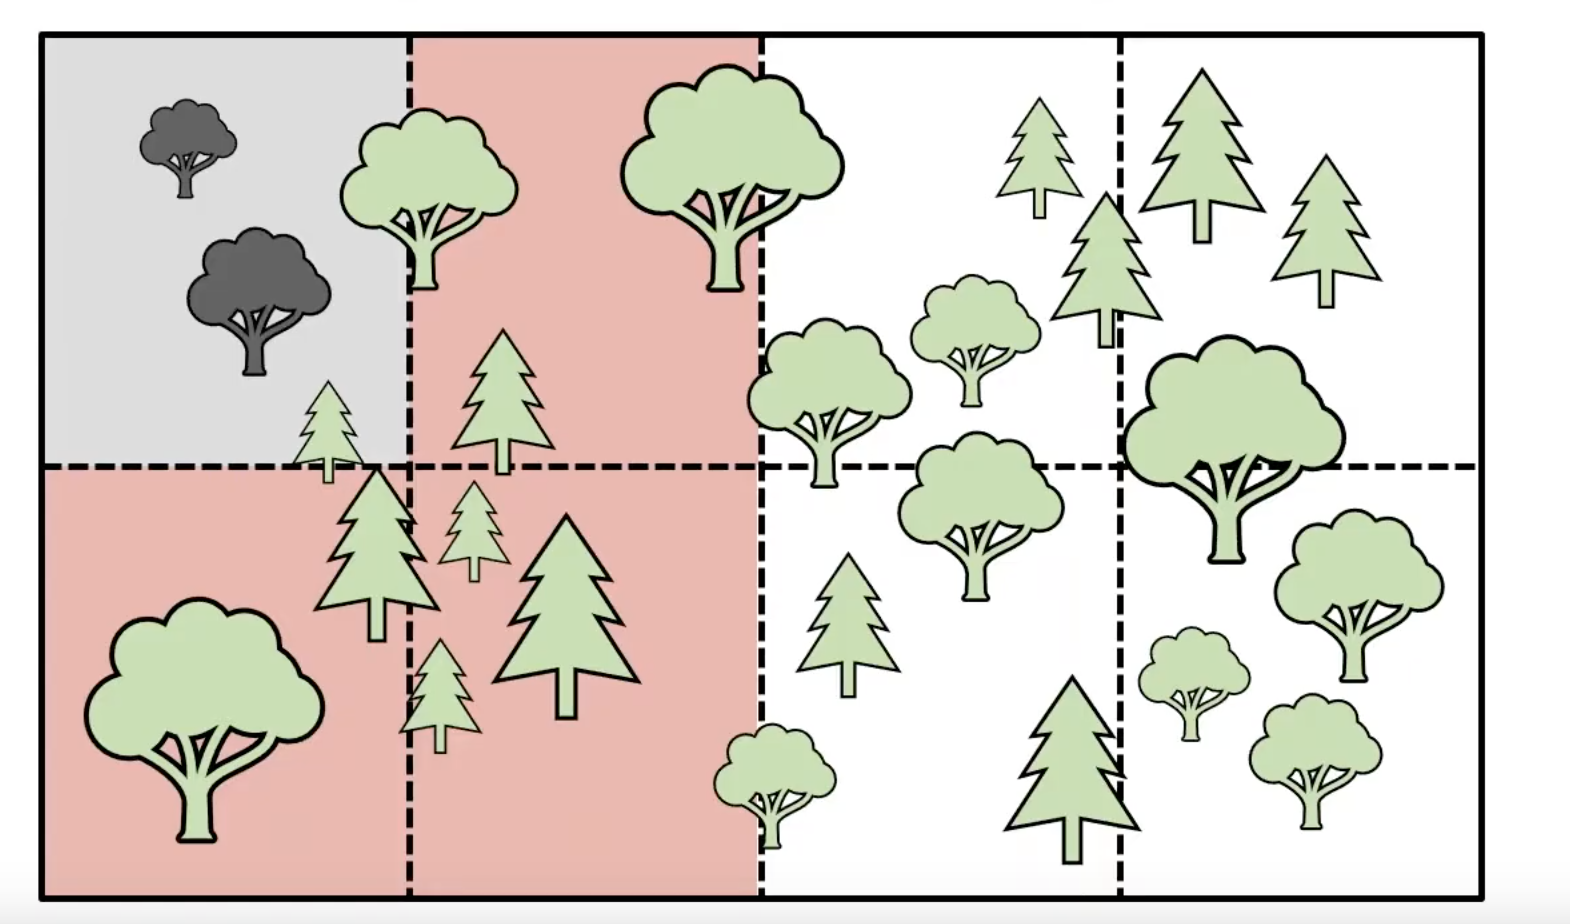
\includegraphics[scale=0.4]{figures/spatial_cross/fig14.png}
\\
\tiny
Source: \url{https://www.youtube.com/watch?v=TK_2MIbChb0&ab_channel=CAUSEweb}
 \end{figure}
\end{frame}
%----------------------------------------------------------------------%

\begin{frame}[fragile]
\frametitle{Spatial Prediction}

\begin{figure}[H] \centering
            \captionsetup{justification=centering}
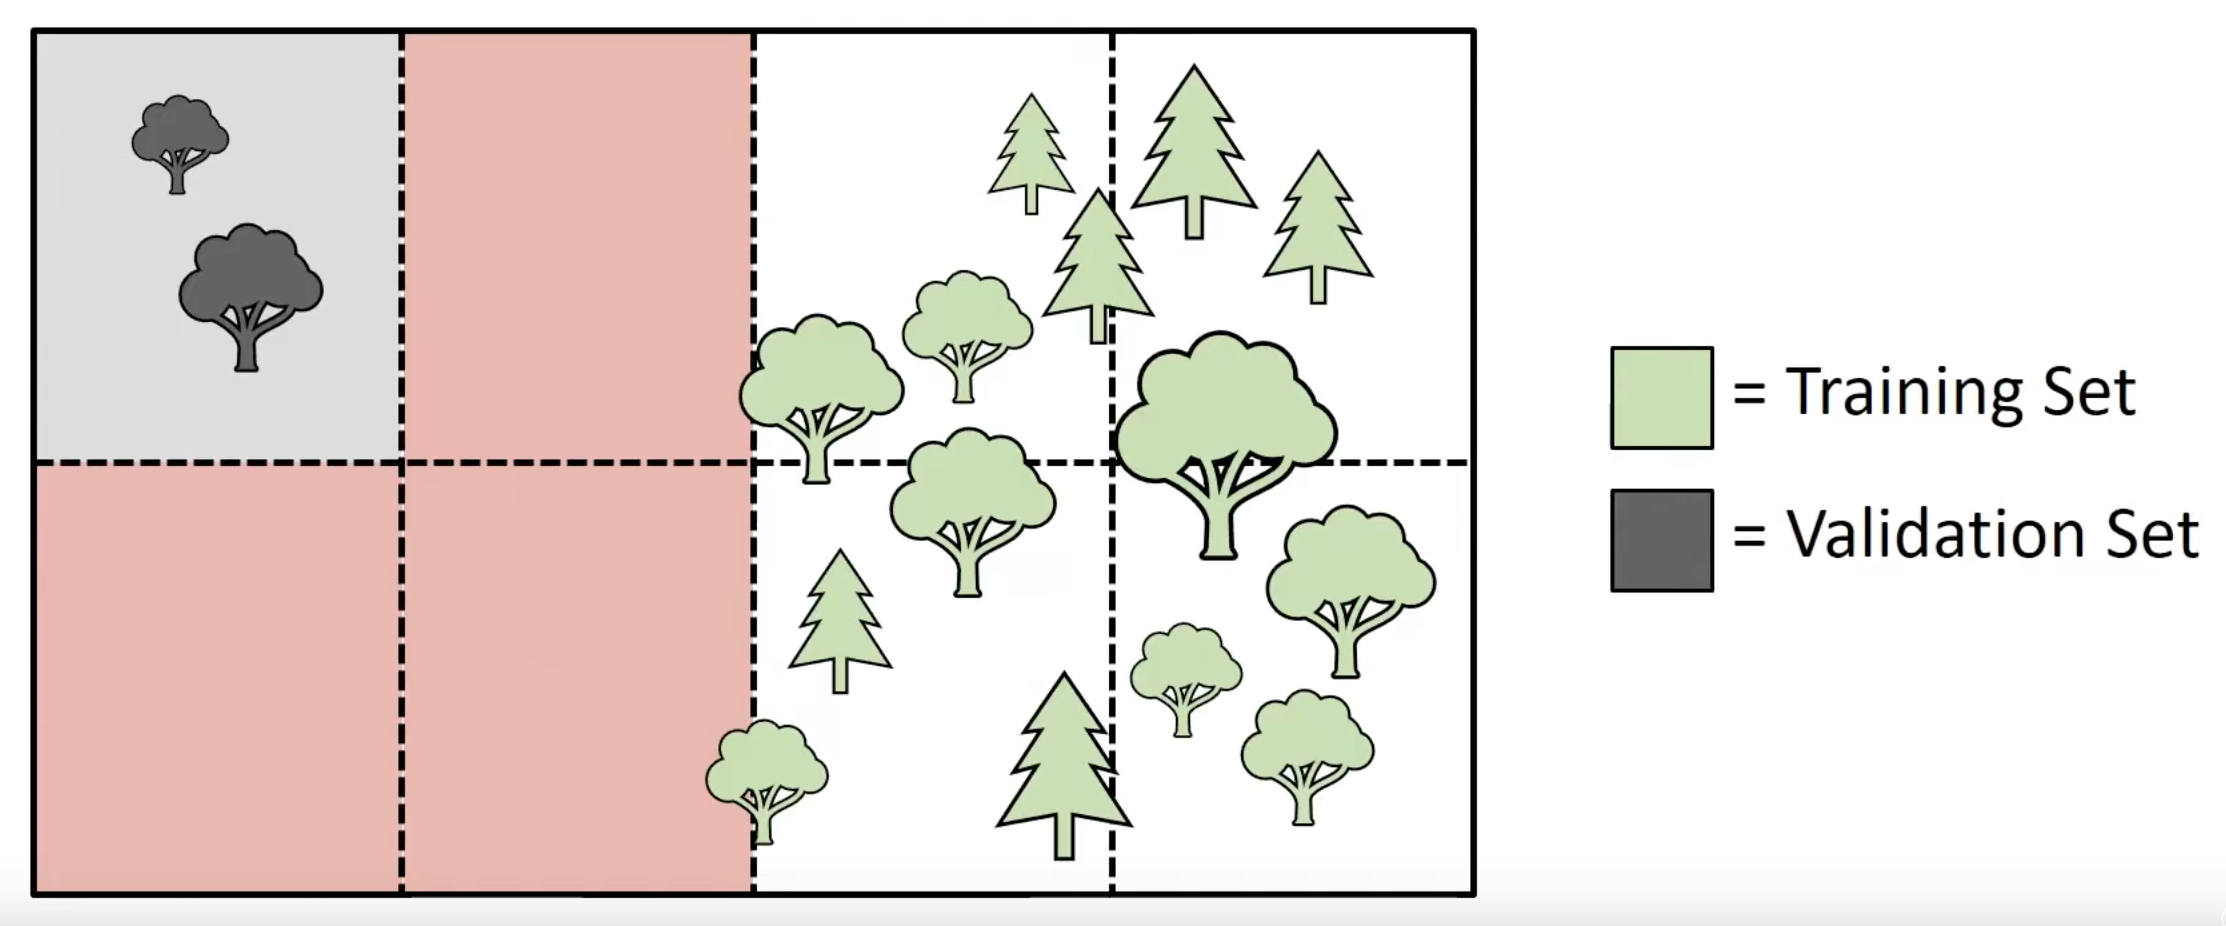
\includegraphics[scale=0.3]{figures/spatial_cross/fig15.png}
\\
\tiny
Source: \url{https://www.youtube.com/watch?v=TK_2MIbChb0&ab_channel=CAUSEweb}
 \end{figure}
\end{frame}
% %----------------------------------------------------------------------%

% \begin{frame}[fragile]
% \frametitle{Spatial Prediction}

% \begin{figure}[H] \centering
%             \captionsetup{justification=centering}
% 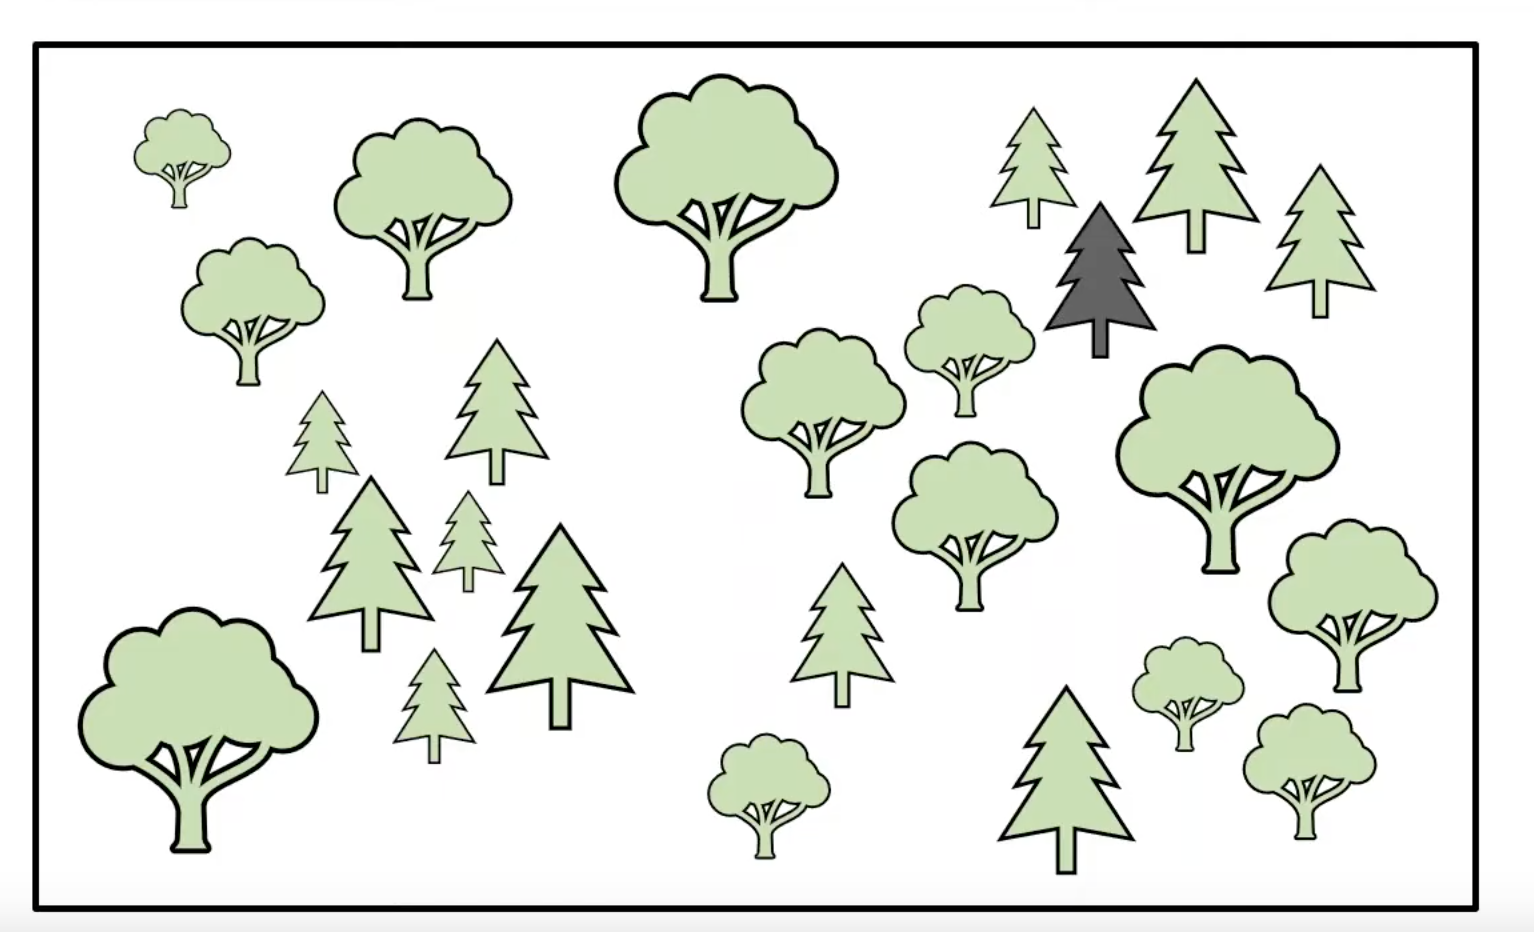
\includegraphics[scale=0.4]{figures/spatial_cross/fig16.png}
% \\
% \tiny
% Source: \url{https://www.youtube.com/watch?v=TK_2MIbChb0&ab_channel=CAUSEweb}
%  \end{figure}
% \end{frame}
% %----------------------------------------------------------------------%

% \begin{frame}[fragile]
% \frametitle{Spatial Prediction}

% \begin{figure}[H] \centering
%             \captionsetup{justification=centering}
% 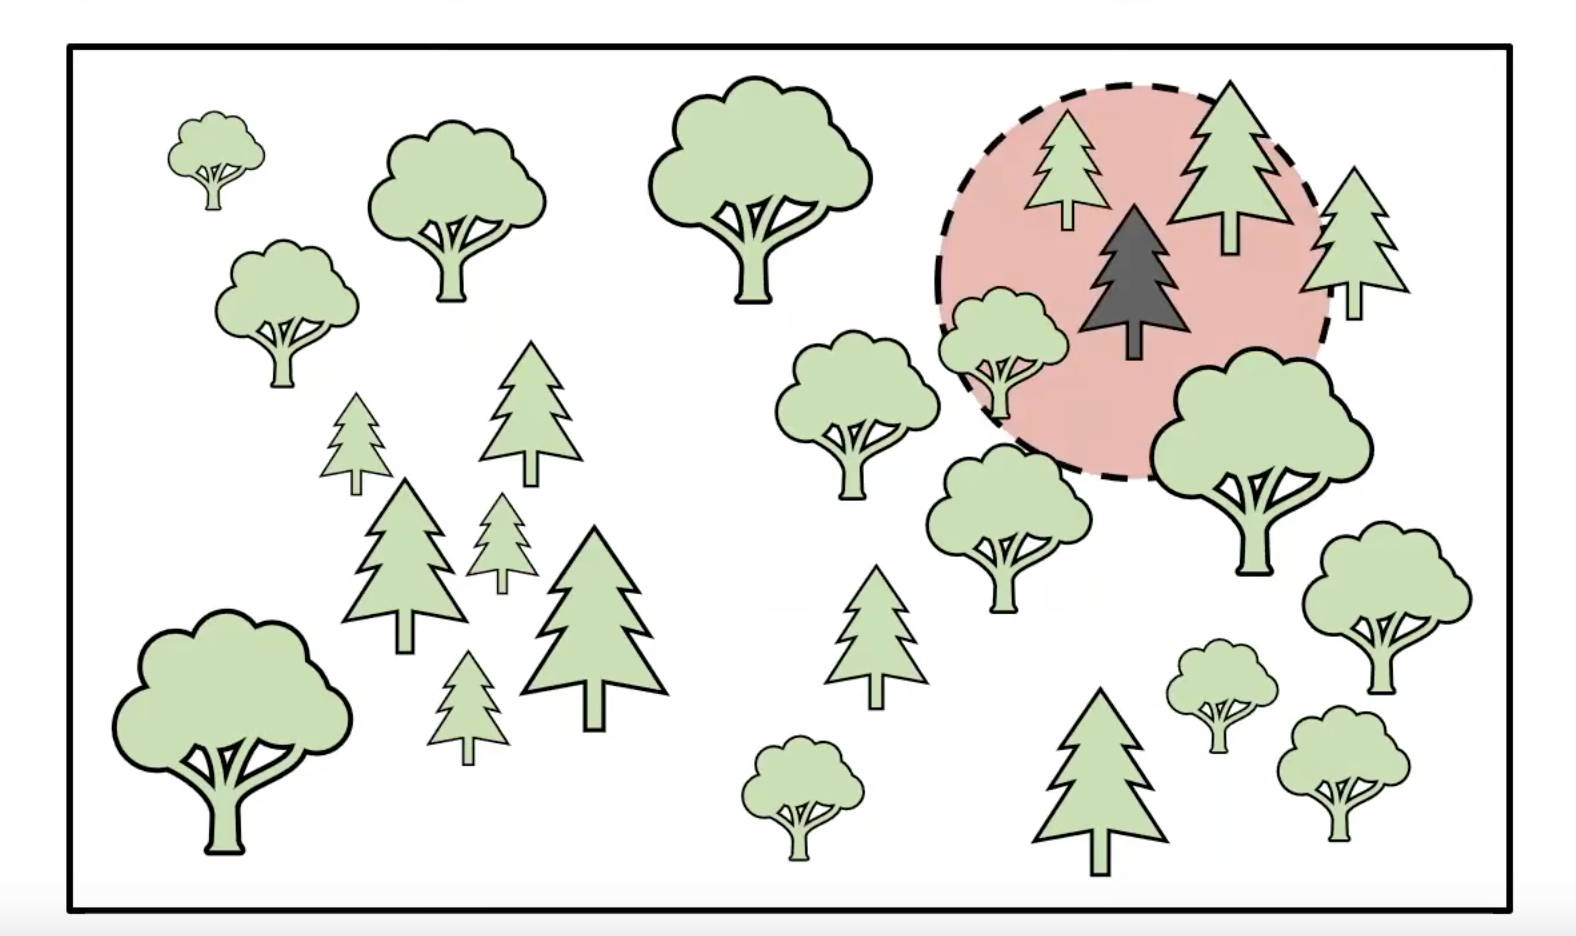
\includegraphics[scale=0.4]{figures/spatial_cross/fig16a.png}
% \\
% \tiny
% Source: \url{https://www.youtube.com/watch?v=TK_2MIbChb0&ab_channel=CAUSEweb}
%  \end{figure}
% \end{frame}
% %----------------------------------------------------------------------%

% \begin{frame}[fragile]
% \frametitle{Spatial Prediction}

% \begin{figure}[H] \centering
%             \captionsetup{justification=centering}
% 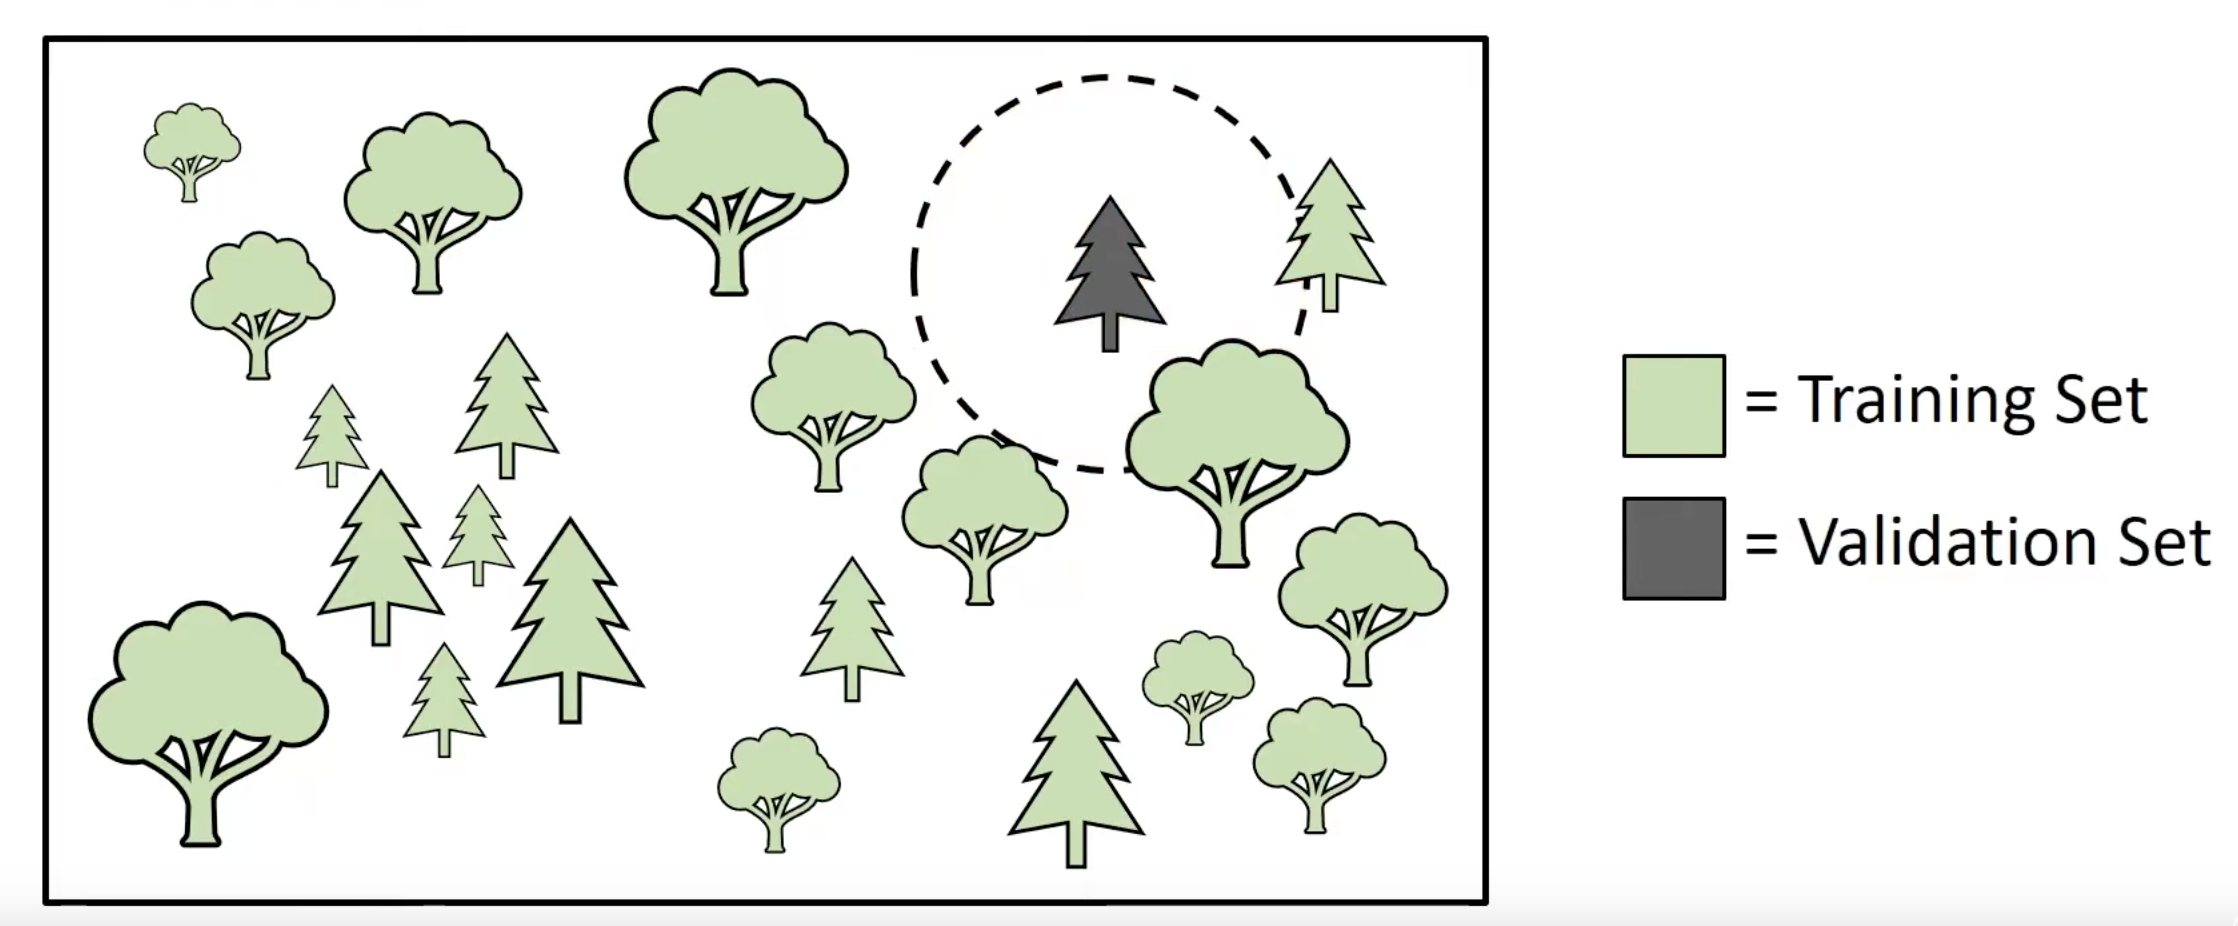
\includegraphics[scale=0.3]{figures/spatial_cross/fig17.png}
% \\
% \tiny
% Source: \url{https://www.youtube.com/watch?v=TK_2MIbChb0&ab_channel=CAUSEweb}
%  \end{figure}



%\end{frame}
%----------------------------------------------------------------------%

%----------------------------------------------------------------------%
%----------------------------------------------------------------------%
\begin{frame}[fragile]
\frametitle{Example: Spatial Cross-Validation}
\begin{figure}[H] \centering
  \centering
  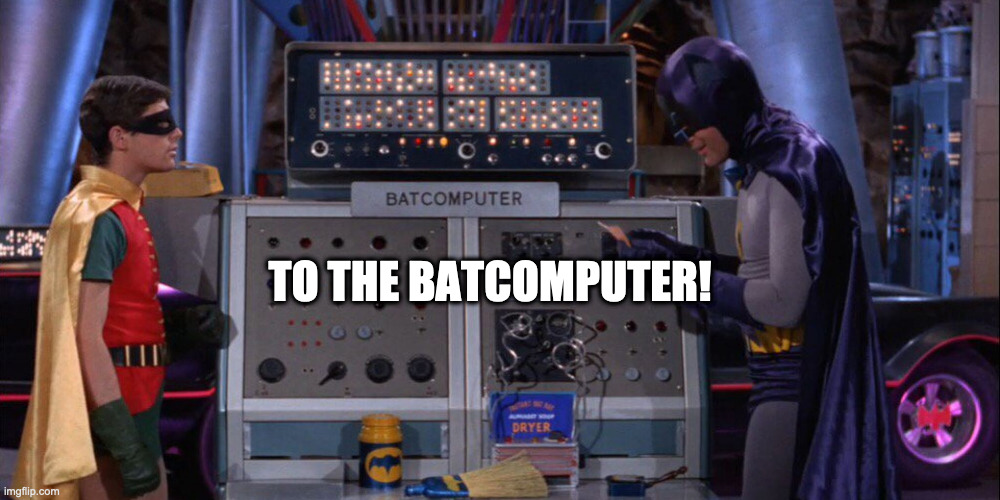
\includegraphics[scale=0.35]{figures/baticomputer_meme.jpg}
  \\
  \tiny photo from \url{https://www.dailydot.com/parsec/batman-1966-labels-tumblr-twitter-vine/}
\end{figure}


\end{frame}

%----------------------------------------------------------------------%
%----------------------------------------------------------------------%
\end{document}
%----------------------------------------------------------------------%
%----------------------------------------------------------------------%

